\documentclass[a4paper,12pt]{article}
\usepackage{titletoc}
\usepackage{letltxmacro}
\usepackage{etoolbox}
\usepackage{lipsum}
\usepackage[utf8]{inputenc}
\usepackage{floatrow}
\usepackage{graphicx}
\usepackage{caption} 
\floatsetup[figure]{style=simple,subcapbesideposition=top}
\captionsetup[figure]{labelfont={color=ao}}
%\usepackage[caption=false,labelformat=simple]{subfig}
  % "labelformat=simple" removes the parenthesis from the caption label
\renewcommand\thesubfigure{\alph{subfigure})}
  % This one adds parenthesis to the display format

\usepackage{graphicx,float}
\usepackage{siunitx}
\captionsetup[subfloat]{labelformat=simple}
\usepackage[subrefformat=parens,labelformat=parens]{subfig}
\setcounter{tocdepth}{1}
\usepackage{spverbatim}
\usepackage{booktabs} % for better table rules
\usepackage{tabularx} % for better column widths
\usepackage{siunitx} % for decimal alignment
\sisetup{table-format=2.2} % set number format
\usepackage{cite}
\usepackage[titletoc]{appendix}
\usepackage[toc,page]{appendix}
\usepackage[section]{placeins} 
\usepackage{amsfonts}
\usepackage{bbm}
\usepackage[section]{placeins}

\usepackage[utf8]{inputenc}
\usepackage[nodisplayskipstretch]{setspace}
\setstretch{1.5}
\graphicspath{{images/}}
\usepackage{parskip}
\usepackage{color}
\usepackage{outline}
\usepackage[normalem]{ulem}
\usepackage{xcolor}
\usepackage{braket}
\usepackage[margin=2cm]{geometry} % Adjust margins
\usepackage{booktabs} % For better-looking tables
\usepackage{array} % For custom column width

\usepackage{cite}
\usepackage[bottom]{footmisc}
\usepackage{enumerate}
\usepackage[T1]{fontenc}
\usepackage{newtxmath,newtxtext}
\usepackage{vmargin}
%\setmarginsrb{leftmargin}{topmargin}{rightmargin}{bottommargin}{headheight}{headsep}{footheight}{footskip}
\setmarginsrb   {20mm}      {20mm}     {20mm}       {20mm}        {10pt}     {10mm}    {0pt}       {0mm}
\usepackage{libertine}
\usepackage{etoolbox}	
\makeatletter
% \patchcmd{<cmd>}{<search>}{<replace>}{<success>}{<failure>}
% --- Patch \chapters

\makeatother
% Set new lengths
\newlength{\chapheadtopskip}\setlength{\chapheadtopskip}{0pt}
\newlength{\chapheadsep}\setlength{\chapheadsep}{20pt}
\newlength{\chapheadbelowskip}\setlength{\chapheadbelowskip}{15pt}
\graphicspath{{images/}}
\usepackage{parskip}
\usepackage{color}
\usepackage{outline}

\usepackage{braket}
\usepackage{helvet}
\renewcommand{\familydefault}{\sfdefault}
\usepackage{cite}
\usepackage[bottom]{footmisc}

\usepackage{enumerate}
\usepackage{vmargin}
\usepackage{hyperref}	% Needed for \url macro in bibliography
% Make hyperlinks a bit nicer:
%\definecolor{ao}{rgb}{0,0,.7}
\definecolor{ao}{rgb}{0,0,0.5}
\definecolor{cadmiumgreen}{rgb}{0.0, 0.42, 0.24}
%\definecolor{ao}{rgb}{0.74, 0.2, 0.64}
\hypersetup{colorlinks=true, breaklinks=true, linkcolor=ao, menucolor=ao, urlcolor=ao, citecolor=ao}
\newcommand{\comm}[1]{ 
\usepackage{fancyhdr}
\pagestyle{fancy}}
%\renewcommand{\chaptermark}[1]{\markboth{#1}{}}
\usepackage{fourier-orns}
\renewcommand\headrule{\hrulefill
\raisebox{-2pt}[10pt][10pt]{\quad\decofourleft\decotwo\decofourright\quad}\hrulefill}
\newcommand{\comm}[1]{ 
\fancyfoot[C]{\thepage}
\rhead{\emph{S365452}}
\lhead{\emph{Maheshwor Tiwari}}}

%\fancyhf{}
%\lhead{\thetitle}
%\cfoot{\thepage}

%% A nice Angstrom symbol
\usepackage{amsmath}
\usepackage{apacite}
\def\angstrom{{\rm\AA}}
\begin{document}
\newcommand{\comm}[1]{ 
\begin{titlepage}
	\thispagestyle{empty}
	\newcommand{\HRule}{\rule{\linewidth}{0.1mm}}
	\centering
	\textbf{\large CHARLES DARWIN UNIVERSITY }\\[.2cm]
	\centering Sydney Campus
	\vspace{6mm}
	\begin{minipage}{0.82\textwidth}
	\begin{center} %\large
	\includegraphics[width=100mm]{cdu.jpeg}%[.1cm]
	\end{center}
	\end{minipage} \\[.3cm]
	\vspace{9mm}
	\begin{center}
	\textsc{\large  ASSIGNMENT ONE }\\[1cm]
	\end{center}
	\HRule \\[0.4cm]
	\begingroup
	\begin{center}
	
\fontfamily{phv}\fontsize{20}{20}\selectfont
 \textbf{\textcolor{ao}{Nanomaterial}}.
 \end{center}
\endgroup
	%{ \large \textbf{\textcolor{blue}{Electronic and transport properties of two-dimensional heterostructures based on graphene and transition metal dichalcogenides}}}\\[0.1cm]
	
	\HRule \\[.2cm]
\begin{minipage}[t]{0.28\textwidth}
\begin{flushleft} 
\centering \emph{Submitted by:}\\
{\color{ao}Maheshwor Tiwari} {\color{ao}Student No.: S365452}
\end{flushleft}
\end{minipage}
\\[2cm]

%\vfill
\large \textit{An assignment presented as part of the Master of Data Science's\\ }\\[0.3cm] % University requirement text
\textit{(SDASC2-2024)}\\[0.4cm]
\centering
\text{S124 PRT574 SECURITY ASSESSMENT IN SOFTWARE DEVELOPMENT }	\\[0.4cm]
		
%\begin{minipage}{0.25\textwidth}
	%\begin{flushright} %\large
	%\centering
	%\includegraphics[width=80mm]{Ini.png}
	%\end{flushright}
	%\end{minipage}	
\begin{minipage}{0.25\textwidth}
	\begin{flushright} %\large
	\end{flushright}
	\end{minipage}
\begin{center}
\today
\end{center}

\end{titlepage}}
\begin{figure}[t]
\centering
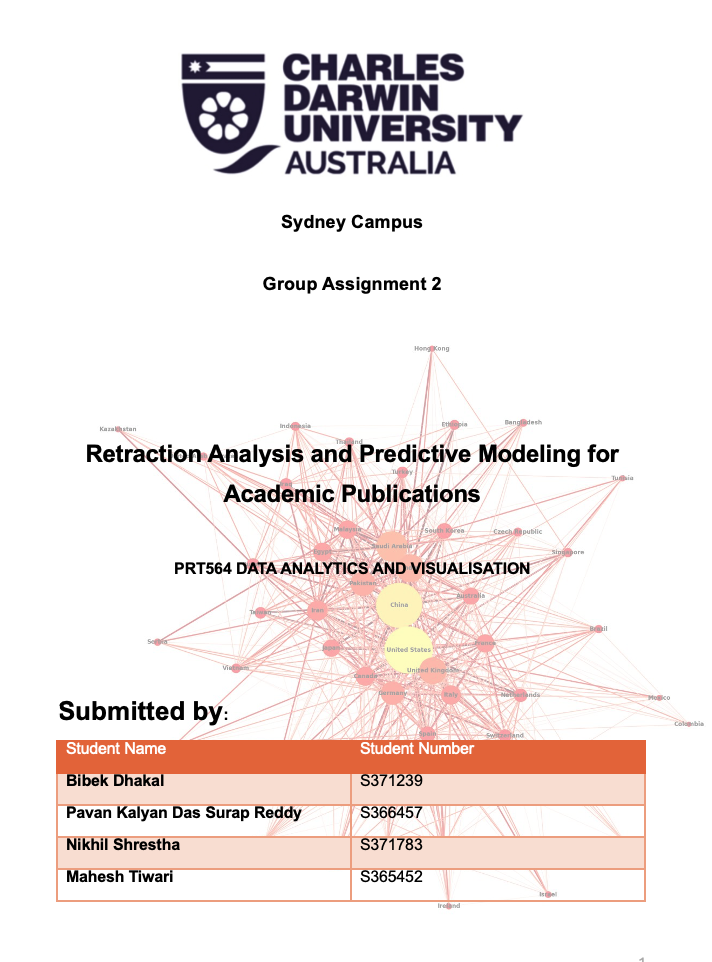
\includegraphics[width=1\linewidth]{tittle.png}
\end{figure}
\clearpage
\newpage

\pagenumbering{arabic}
\setcounter{page}{1}
\dominitoc
\pagebreak
\setcounter{tocdepth}{2}
\setcounter{secnumdepth}{3}
\newcommand{\comm}[1]{ }
\renewcommand{\thesection}{\arabic{section}}
\tableofcontents
\thispagestyle{empty}
\newpage
\setcounter{page}{1}
\newcommand{\comm}[1]{ }
\newpage





\begin{document}

\clearpage
\newpage

\listoffigures
\clearpage
\newpage

\section{Introduction}
The retraction of research papers involves academic publishers removing their previously published papers from circulation. Various scientific errors or instances of academic misconduct can lead to retractions such as controversial claims that 5G technology causes COVID-19 infections (Retraction Watch, n.d.) or the notorious study linking vaccines to autism in children (Godlee, 2011). In 2023, there was a record high of over 10,000 retractions in a single year, indicating a potential rise in questionable scientific practices (Van Noorden, 2023). Meanwhile, governments are increasingly using scientific evidence to shape laws and regulations as seen in responses to the COVID-19 pandemic. Therefore, the growing number of retractions is alarming because flawed science can result in flawed public policies.

Understanding the factors behind past retractions can help prevent or reduce poor practices in science. This project brief outlines the main data analytics objectives for the PRT564 group project including a description of the primary dataset (Retraction Watch, n.d.).

\section{Data Preparation and Initial Analysis}
The retraction records dataset initially contained 35,215 records with 21 columns. Notably, a significant portion of the dataset contained null values in certain columns: 43.3\% of the records had null values in the 'URLS' column, 70.2\% in the 'Notes' column, and smaller percentages in columns like 'RetractionDOI' and 'Paywalled.' To streamline the analysis, redundant columns such as 'Record ID', 'URLS', 'OriginalPaperDOI', 'RetractionDOI', 'RetractionPubMedID', 'OriginalPaperPubMedID', and 'Notes' were removed. Additionally, duplicate rows and rows with null values in the 'Paywalled' column were eliminated, resulting in a final cleaned dataset of 35,184 records and 12 columns. This indicates a minor reduction in the number of records due to cleaning.

\section{Feature Engineering}
Next, the Original Paper Date and Retraction Date columns were transformed into a DateTime format allowing for calculating the Time Difference in Days which measures the number of days between an original paper's publication and its retraction. Time differences range from 1 day to 1344 days. Two new ratio columns were created: Retraction to Citation Ratio and Citation to Retraction Ratio. These ratios provide insights into the relationship between retraction timings and citation counts. To avoid mathematical errors, zero values in Time Difference in Days and Citation Count were adjusted to 1 and 1.1 respectively.

\section{Transforming the Subject Column}
The Subject column was transformed to show sorted unique subjects within each entry improving the clarity and consistency of subject data. For example, entries like 'B/T PHY', 'PHY', and 'BLS ENV HSC' indicate multiple subjects associated with each paper. Unique occurrences of subjects identified include 'B/T', 'BLS', 'ENV', 'HSC', 'HUM', 'PHY', and 'SOC.' This standardization allows for accurate counting and analysis of subject occurrences within the dataset.

\section{Top 10 Most Frequently Occurring Entries in Various Column}

\subsection{Most Frequent Subjects}
\begin{figure}[h]
    \centering
    \includegraphics[width=0.8\textwidth]{top_10_subject.png}
    \caption{Top 10 Most Frequently Occurring Subject}
    \label{fig:subject_frequency}
\end{figure}

Figure \ref{fig:subject_frequency} shows that the majority of retracted papers fall under Biological Sciences (BLS) with over 13,000 occurrences, Biotechnology/Technical Sciences (B/T) with nearly 12,000 occurrences, and Health Sciences (HSC) with just over 10,000 occurrences. These high numbers suggest that these fields, likely due to their high research output, face more scrutiny and potential issues leading to retractions. Fields like Physics (PHY) and Social Sciences (SOC) also show significant numbers but to a lesser extent indicating a broader distribution of retractions across different scientific domains.


\subsection{Most Frequent Journals}
\begin{figure}[h!]
    \centering
    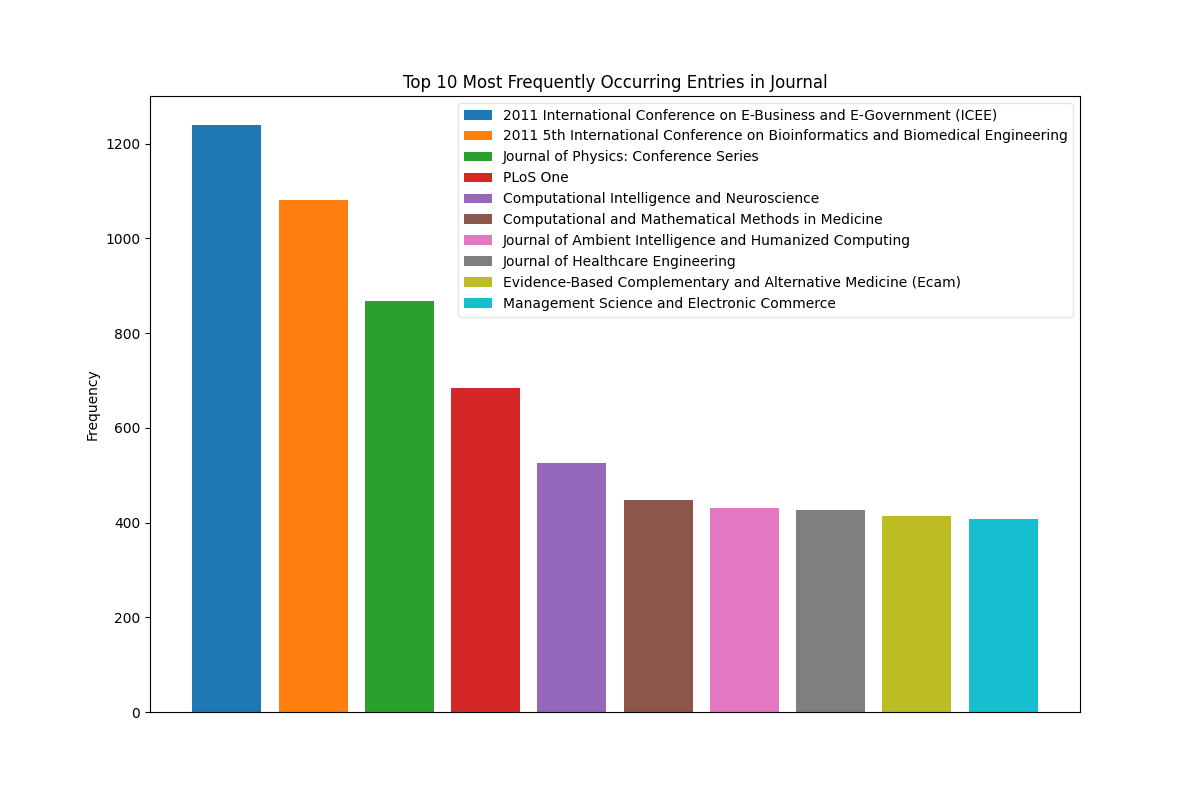
\includegraphics[width=0.8\textwidth]{top_10_Journal.png}
    \caption{Top 10 Most Frequently Occurring Journals}
    \label{fig:journal_frequency}
\end{figure}

Figure \ref{fig:journal_frequency} indicates that retractions are highly concentrated in certain journals, particularly conference proceedings and multidisciplinary journals. For instance, "2011 International Conference on E-Business and E-Government (ICEE)" has over 1,200 retractions and "PLoS One" has 685 retractions. This reflects the extensive research output and possibly less stringent review processes in these venues. The presence of specialized journals like "Journal of Physics: Conference Series" and "Computational Intelligence and Neuroscience" underscores the prevalence of retractions in specific research communities. Notably, there are 5,835 unique journal titles in the dataset highlighting a wide diversity in publication sources.

\subsection{Most Frequent Publishers}
\begin{figure}[h!]
    \centering
    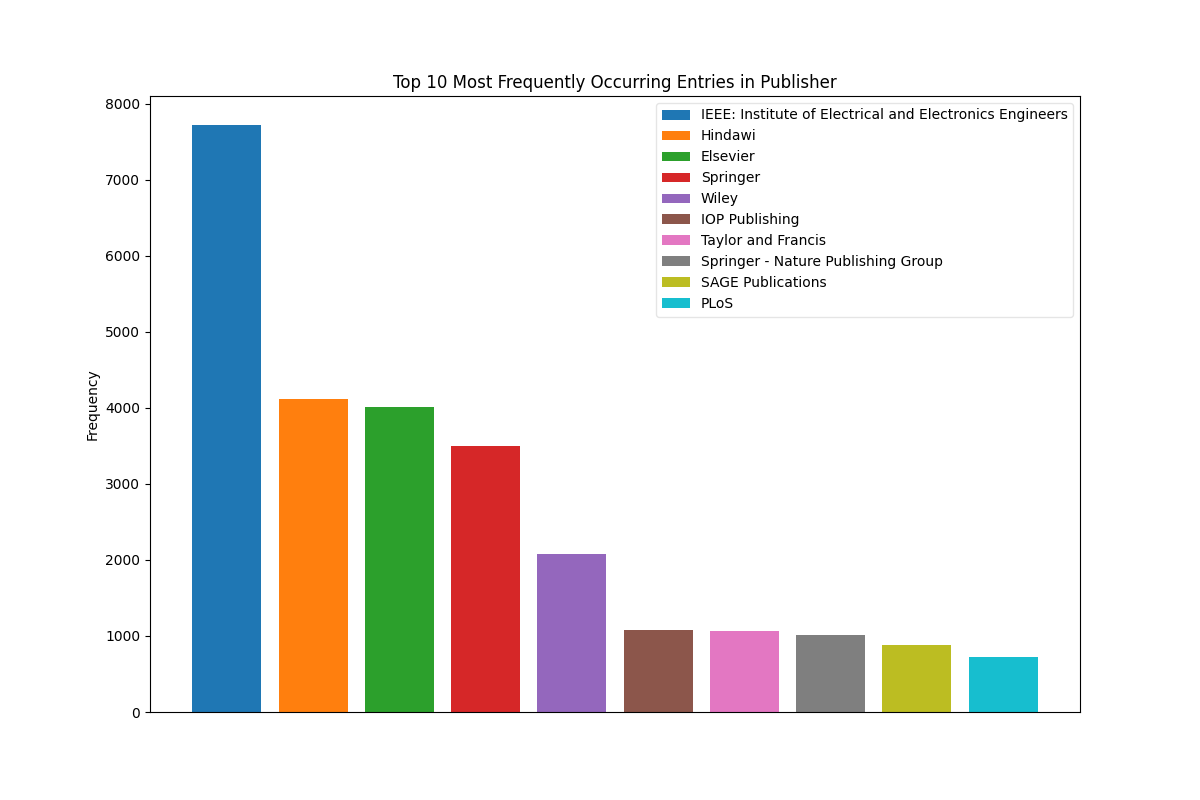
\includegraphics[width=0.8\textwidth]{top_10_Publisher.png}
    \caption{Top 10 Most Frequently Occurring Publishers}
    \label{fig:publisher_frequency}
\end{figure}

Figure \ref{fig:publisher_frequency} reveals that IEEE with over 7,700 retractions, Hindawi (4,115 retractions), and Elsevier (4,019 retractions) are the top publishers with the most retractions. This could be attributed to their large publication volumes. The dominance of IEEE suggests a significant proportion of retractions in engineering and technology fields while Hindawi and Elsevier highlight issues in broader scientific publishing. Notably, Springer (3,499 retractions) and Wiley (2,080 retractions) also appear frequently indicating widespread challenges across various publishers. The dataset includes a total of 608 unique publishers reflecting a broad spectrum of publication sources.

\subsection{Most Frequent Countries}
\begin{figure}[h!]
    \centering
    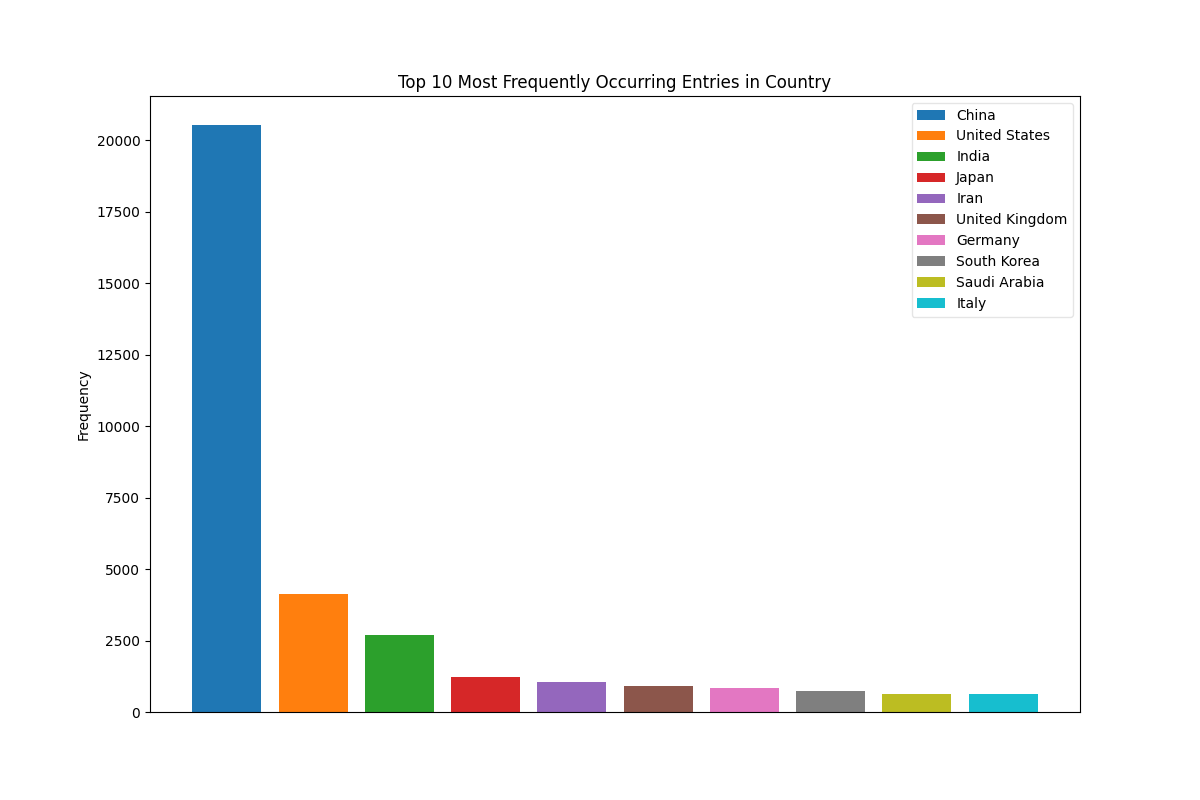
\includegraphics[width=0.8\textwidth]{top_10_Country.png}
    \caption{Top 10 Most Frequently Occurring Countries}
    \label{fig:country_frequency}
\end{figure}

Figure \ref{fig:country_frequency} shows a strikingly high number of retractions from China with over 20,000 occurrences followed by the United States with over 4,100 and India with nearly 2,700 retractions. This might reflect the sheer volume of research output from these countries as well as varying standards of research integrity and pressure to publish. The prominence of countries like Japan, Iran, and South Korea points to regional trends in research practices and potential areas for improvement in publication ethics. There are 167 unique countries represented in the dataset indicating a global scope of retracted research.

\subsection{Most Frequent Article Types}
\begin{figure}[h!]
    \centering
    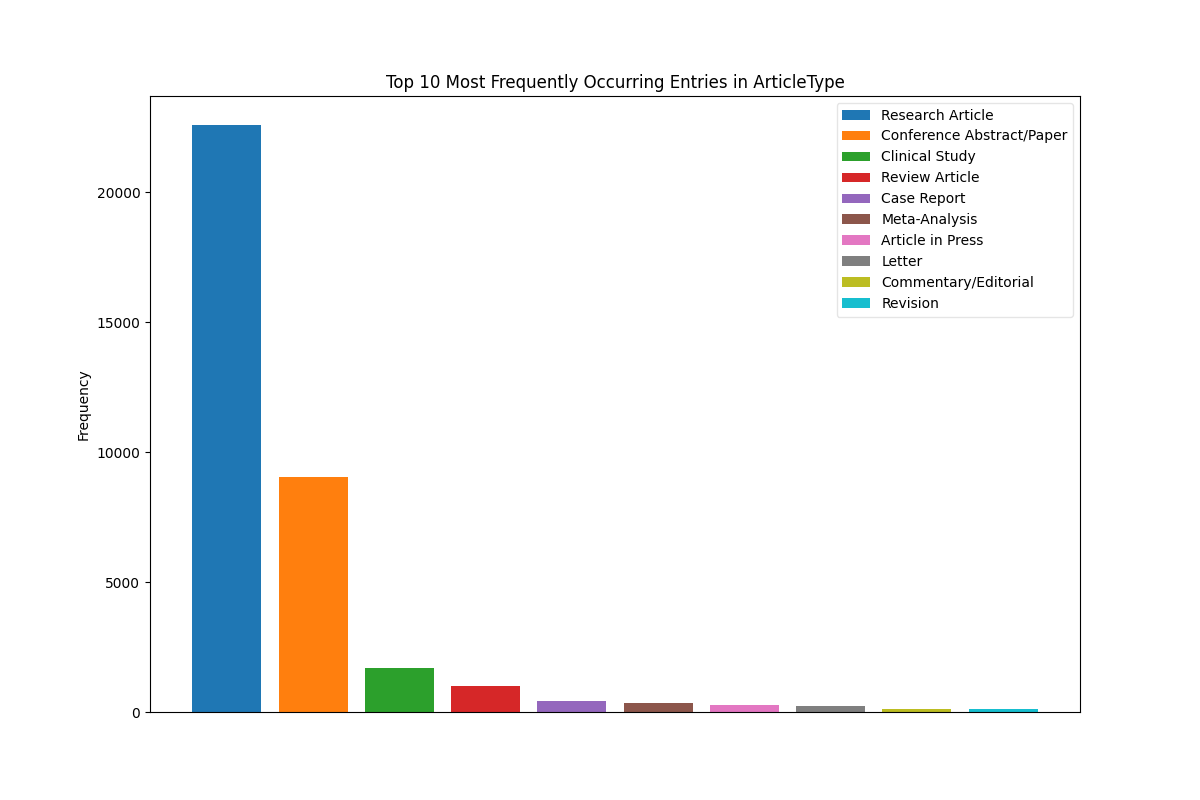
\includegraphics[width=0.8\textwidth]{top_10_ArticleType.png}
    \caption{Top 10 Most Frequently Occurring Article Types}
    \label{fig:article_type_frequency}
\end{figure}

Figure \ref{fig:article_type_frequency} reveals that research articles (over 22,500 retractions) and conference papers (over 9,000 retractions) constitute the majority of retractions. This could be due to the high volume of these article types as well as the complexity and potential for error in original research. Clinical studies, review articles, and case reports also appear highlighting the need for vigilance across different types of scholarly work. The dataset includes 25 unique article types showing a variety of publication formats affected by retractions.

\subsection{Most Frequent Retraction Reasons}
\begin{figure}[h!]
    \centering
    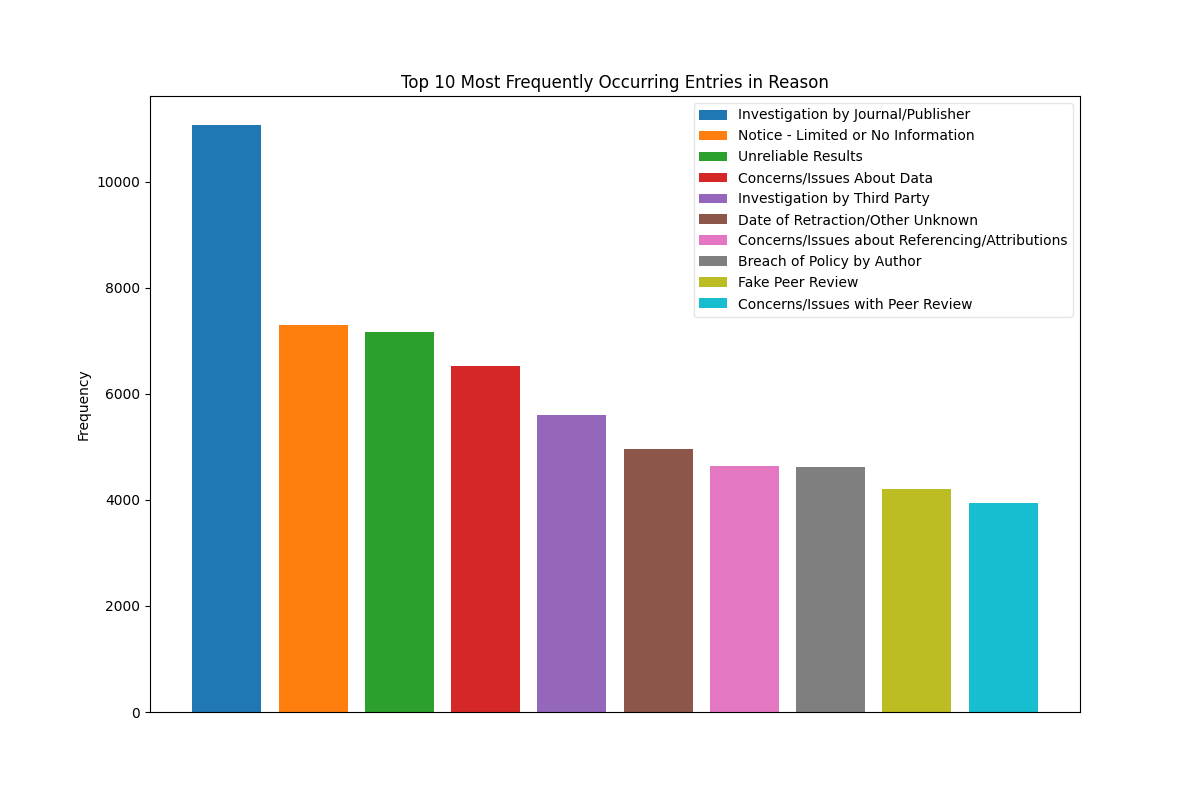
\includegraphics[width=0.8\textwidth]{top_10_Reason.png}
    \caption{Top 10 Most Frequently Occurring Retraction Reasons}
    \label{fig:retraction_reason_frequency}
\end{figure}

Figure \ref{fig:retraction_reason_frequency} underscores the primary reasons for retraction with investigations by journals or publishers (over 11,000 retractions) and unreliable results (7,169 retractions) being the most common. This reflects the crucial role of editorial oversight in maintaining research quality. Issues with data, referencing, and peer review are also significant indicating common pitfalls in the research process that need addressing. There are 108 unique reasons for retraction recorded in the dataset illustrating a wide range of issues leading to retractions.

\subsection{Most Frequent Authors}
\begin{figure}[h!]
    \centering
    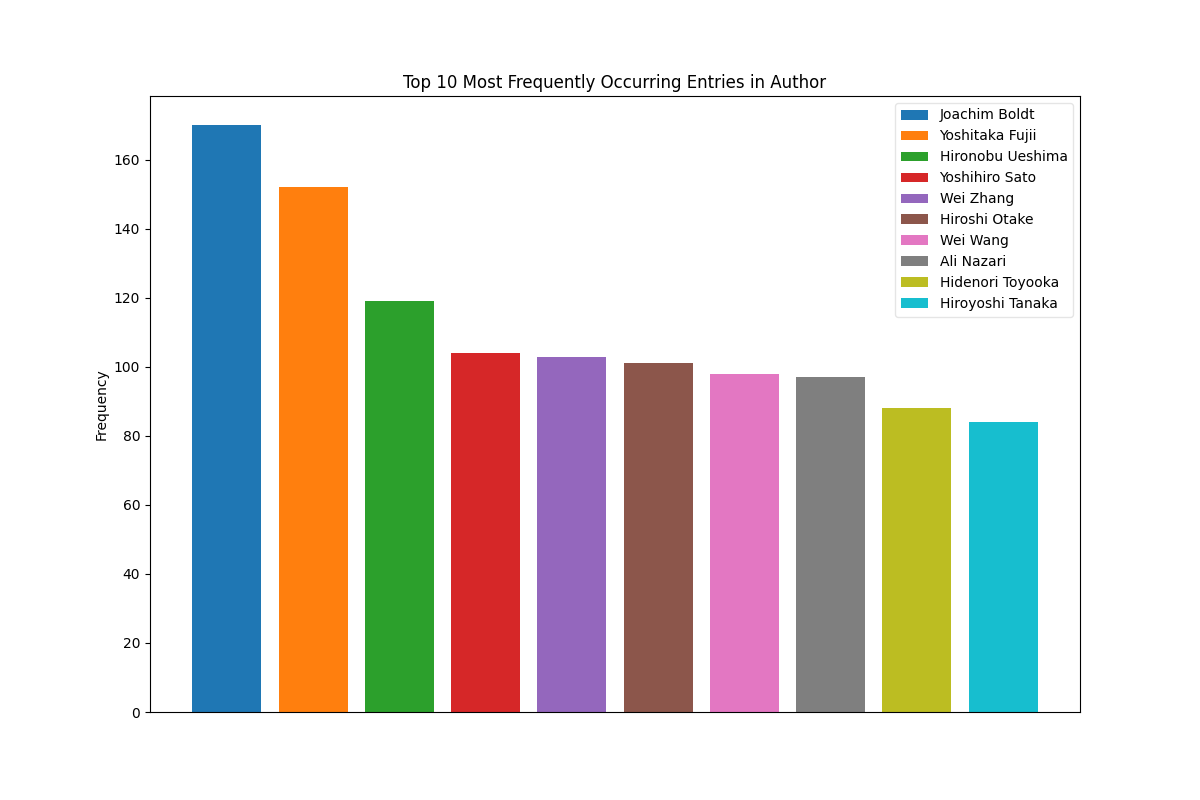
\includegraphics[width=0.8\textwidth]{top_10_Author.png}
    \caption{Top 10 Most Frequently Occurring Authors}
    \label{fig:author_frequency}
\end{figure}

Figure \ref{fig:author_frequency} highlights specific authors with recurrent retractions with Joachim Boldt having 170 retractions and Yoshitaka Fujii with 152 retractions. Such high numbers suggest patterns of problematic research practices and the need for better oversight and accountability in scientific publishing. The dataset includes a staggering 101,341 unique authors indicating the vast number of researchers involved in retracted papers.

\section{Paywalled Frequency Distribution}
\begin{figure}[h!]
    \centering
    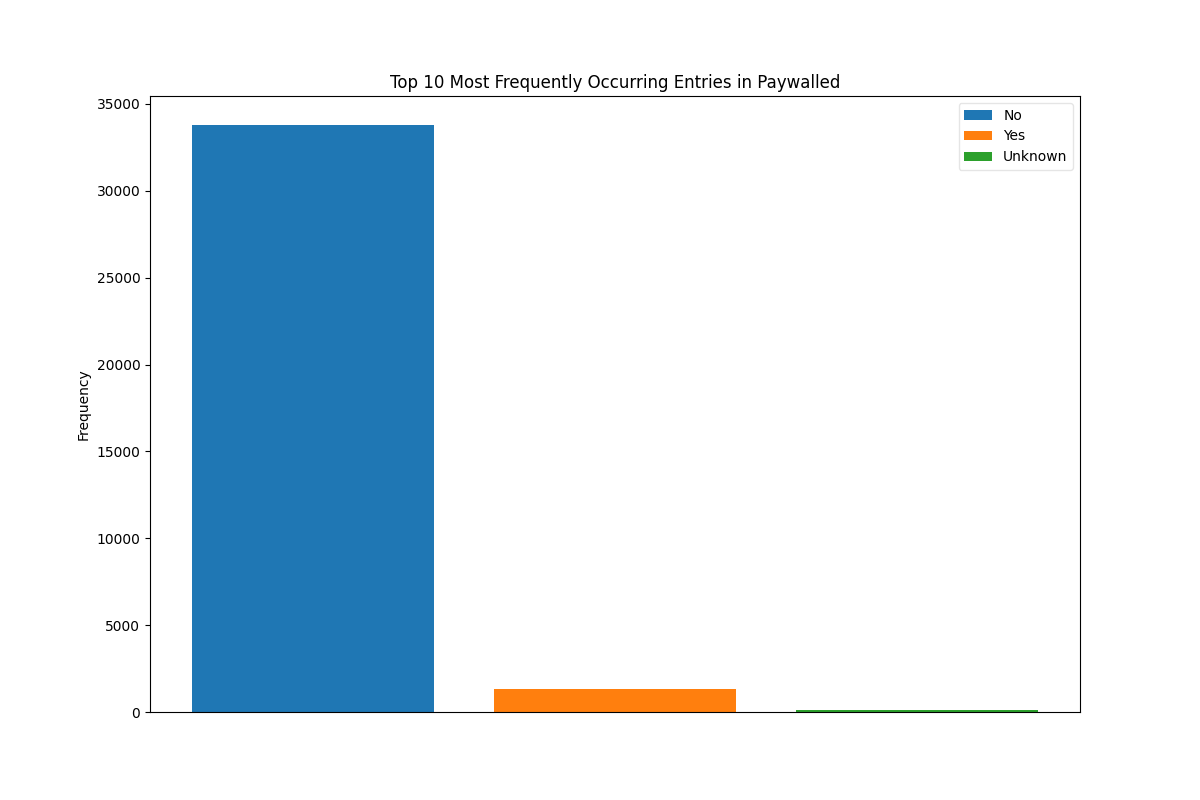
\includegraphics[width=0.8\textwidth]{top_10_Paywalled.png}
    \caption{Paywalled Frequency Distribution}
    \label{fig:paywalled_frequency}
\end{figure}

The bar chart in Figure \ref{fig:paywalled_frequency} visualizes the distribution of retractions based on whether the retracted papers were behind a paywall. The majority of retracted papers (33,766) are not paywalled indicating that these papers were freely accessible to the public. This suggests that open access does not necessarily correlate with higher or lower rates of retractions compared to paywalled articles. A smaller number of retracted papers (1,330) were paywalled meaning access to these papers required a subscription or payment. This could indicate that paywalled journals might have different editorial practices or that the accessibility of papers does not significantly impact the likelihood of retraction. There are 88 instances where the paywall status is unknown a relatively minor category but worth noting for completeness. The data indicates that the majority of retractions occur in non-paywalled journals highlighting the importance of rigorous peer review and editorial standards across all types of publications.


The world map analysis highlights the frequency and percentage of retractions across different countries with China leading significantly at 20,544 retractions (49.33\%) indicating rigorous scrutiny and potential issues in its research outputs. The United States follows with 4,140 retractions (9.94\%) reflecting its substantial contribution to global research and ongoing efforts to maintain integrity. India with 2,679 retractions (6.43\%) shows increased vigilance amid its growing research activities. Japan and Iran accounting for 1,211 (2.91\%) and 1,058 (2.54\%) retractions respectively demonstrate moderate levels of retractions underscoring their focus on upholding research standards. This geographic distribution underscores the global nature of retractions emphasizing the need for robust practices and international collaboration to address research misconduct and enhance the overall quality of scientific literature.
\clearpage

\begin{figure}[h!]
    \centering
    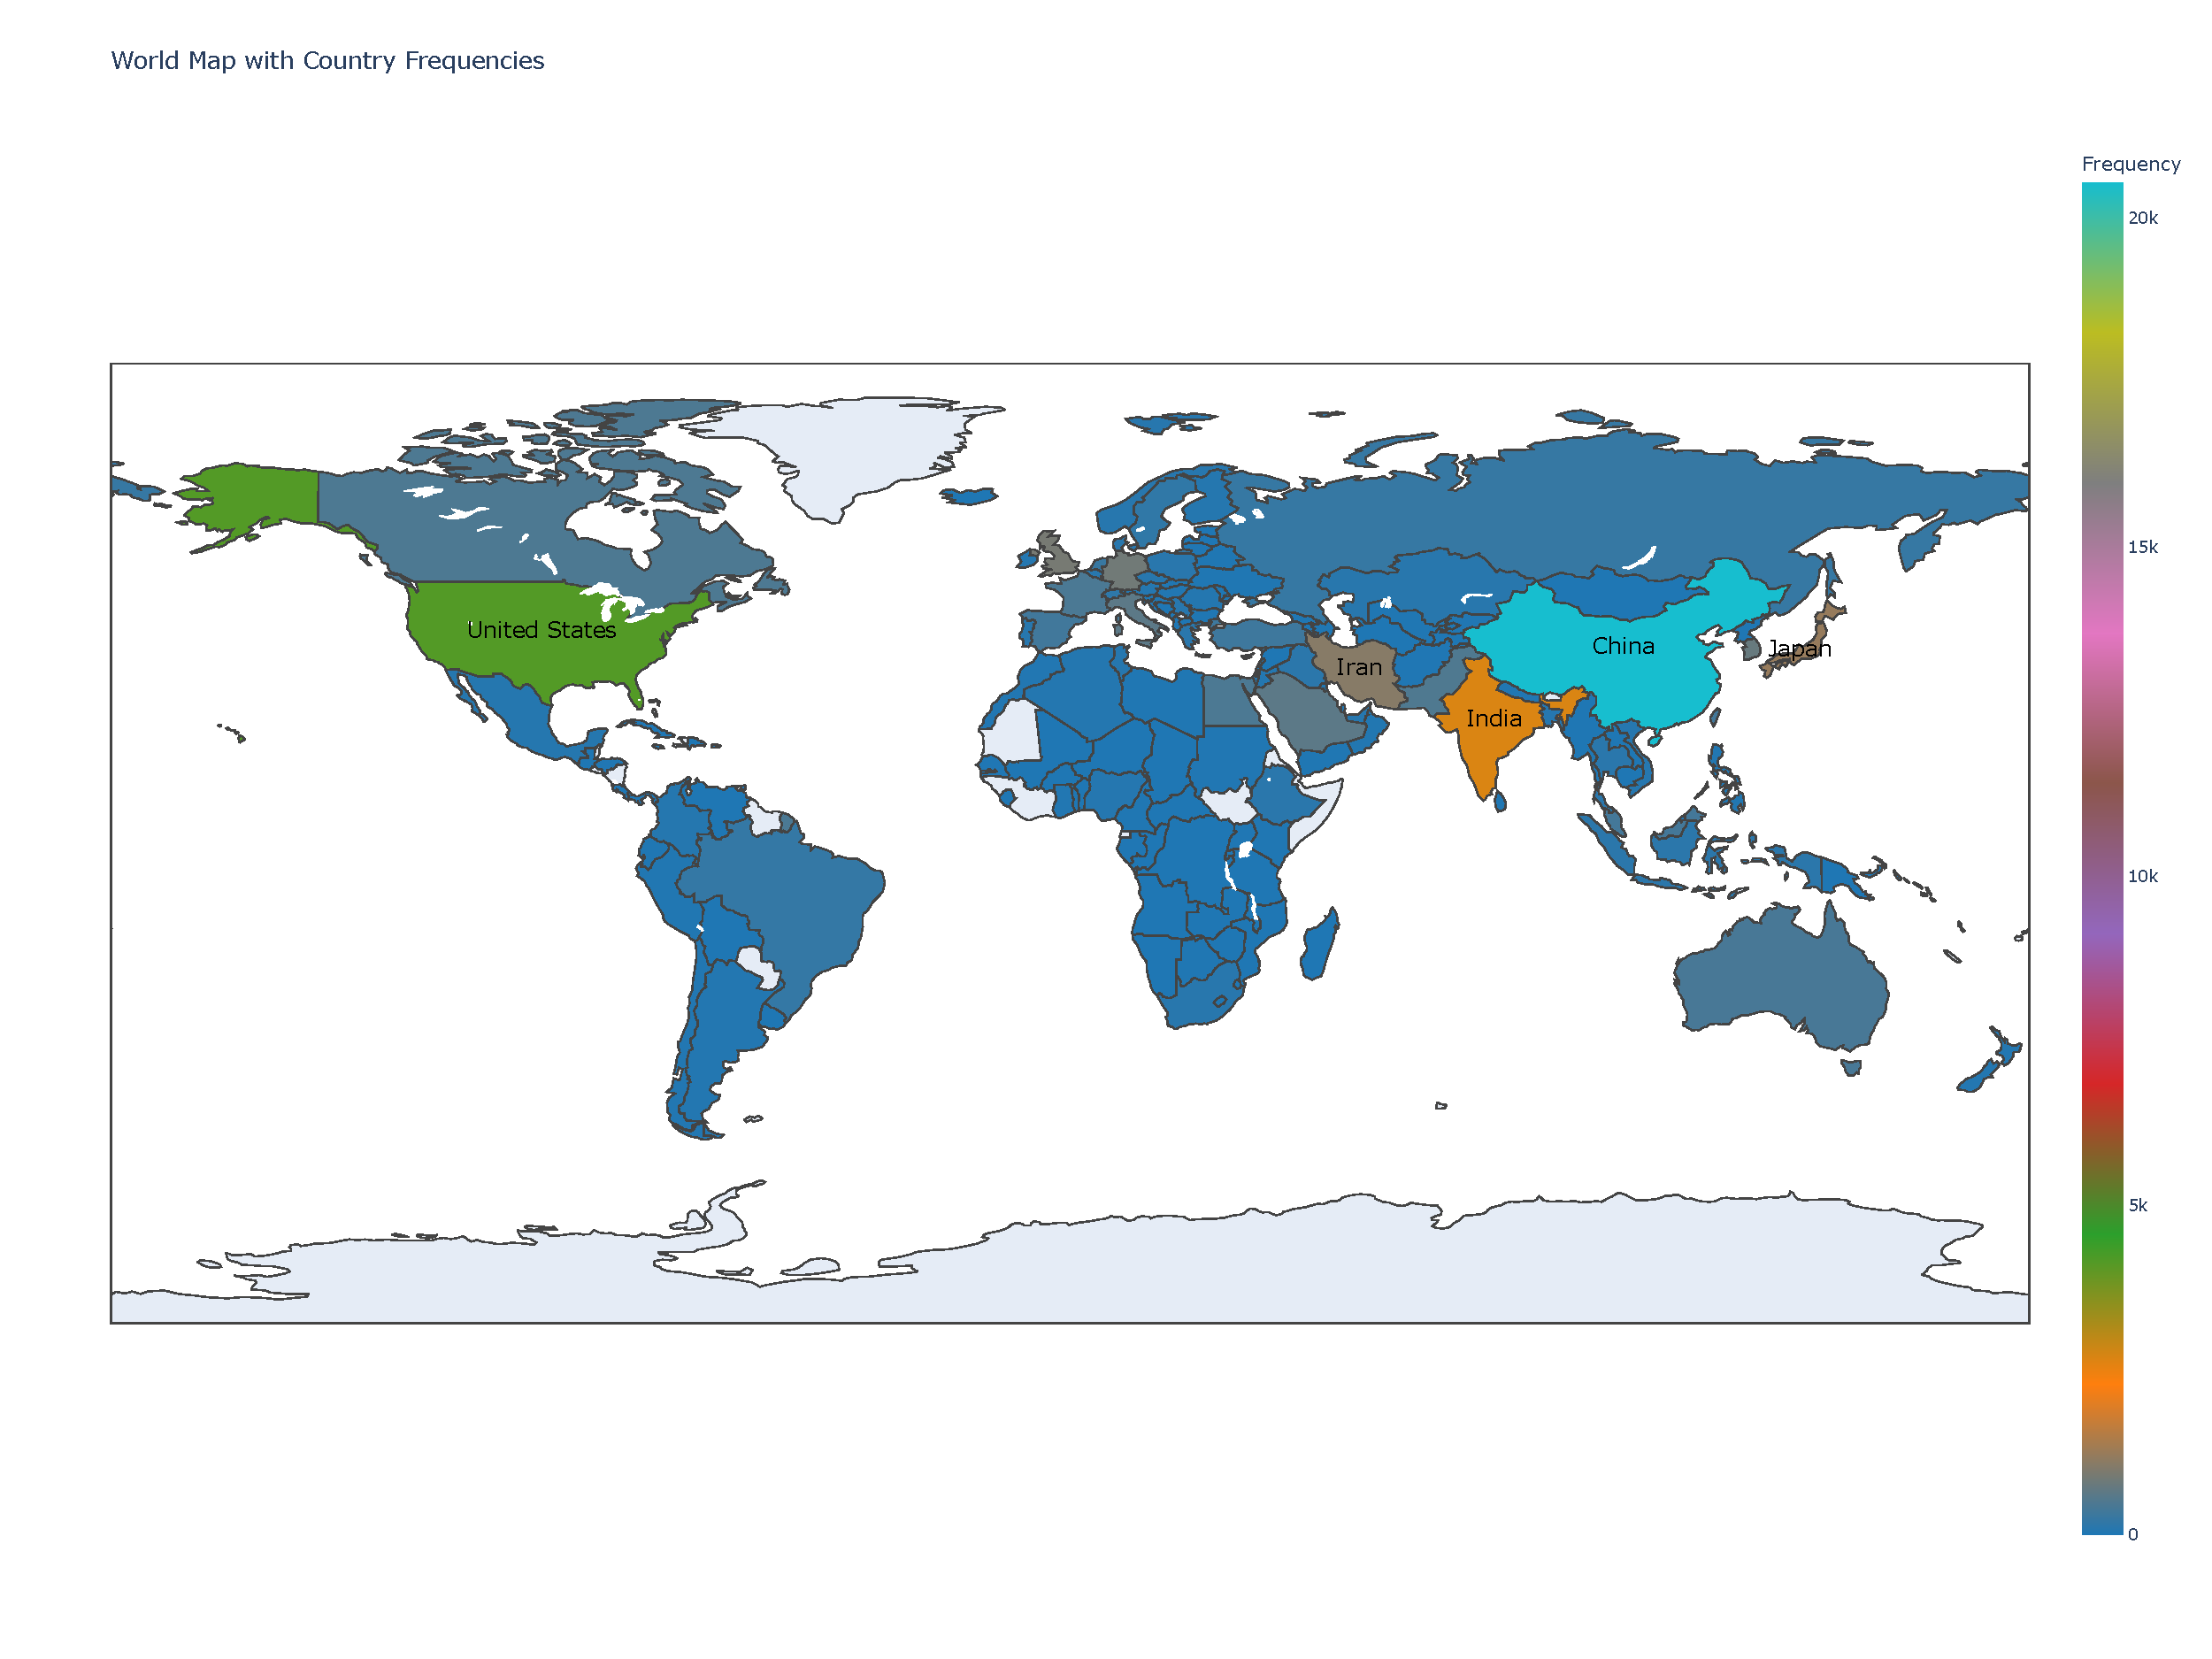
\includegraphics[width=1\textwidth]{world_map_frequencies.pdf}
    \caption{Retraction around the world.}
    \label{fig:worldmap}
\end{figure}


\section{Network Graphs}

\subsection{Network Graph for Retraction Reasons}
\begin{figure}[h!]
    \centering
    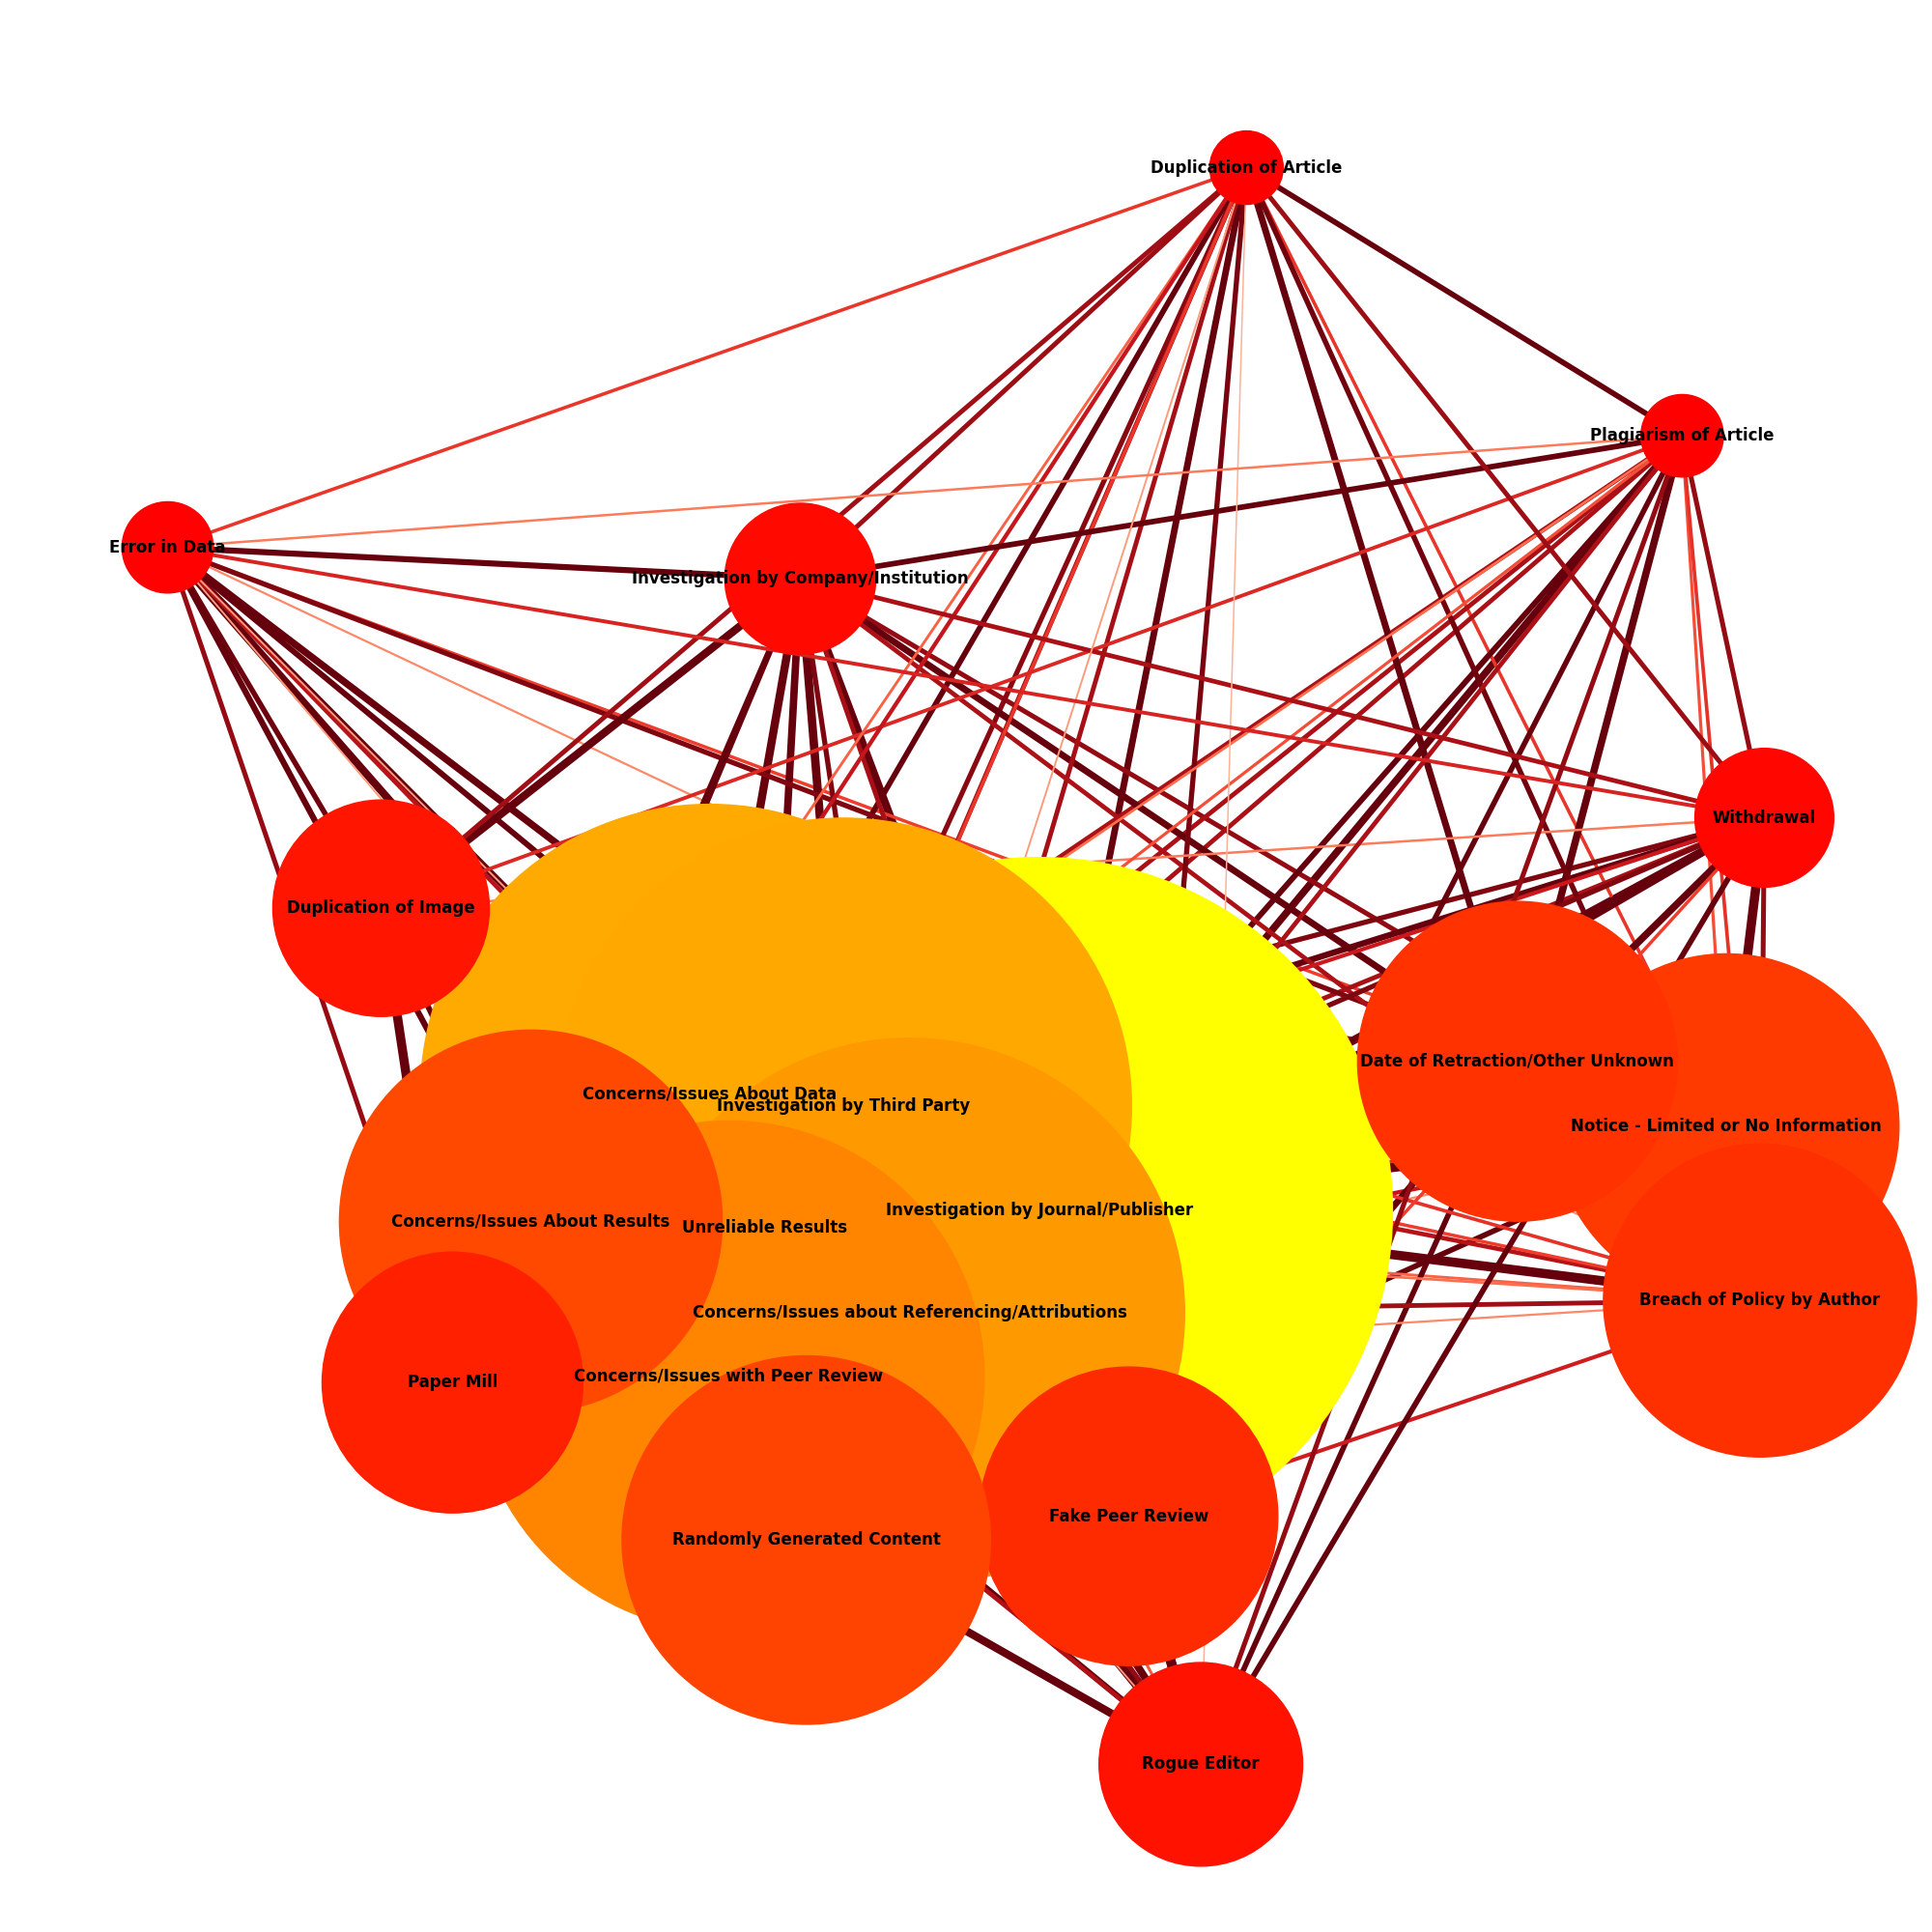
\includegraphics[width=0.8\textwidth]{network_graph_Reason.png}
    \caption{Network Graph for Retraction Reasons}
    \label{fig:retraction_reason_network}
\end{figure}

Figure \ref{fig:retraction_reason_network} visualizes the co-occurrence of different retraction reasons with node sizes representing frequency and edge thickness indicating the strength of co-occurrence between reasons. The weighted degree of each node highlights the centrality of certain reasons within the network. Key observations include the prominence of "Investigation by Journal/Publisher" which is the most central and frequent reason for retractions with a weighted degree of 34,319. "Unreliable Results" (26,253 weighted degree) and "Concerns/Issues About Data" (24,623 weighted degree) are also significant frequently co-occurring with other reasons forming a dense network at the center. Other notable reasons include "Notice - Limited or No Information" (10,387 weighted degree) and "Breach of Policy by Author" (4,618 weighted degree) highlighting common issues related to transparency and author conduct. The graph emphasizes the complex nature of retraction cases where multiple issues are often interlinked necessitating thorough investigation and multi-faceted solutions.

\subsection{Network Graph for Countries}
\begin{figure}[h!]
    \centering
    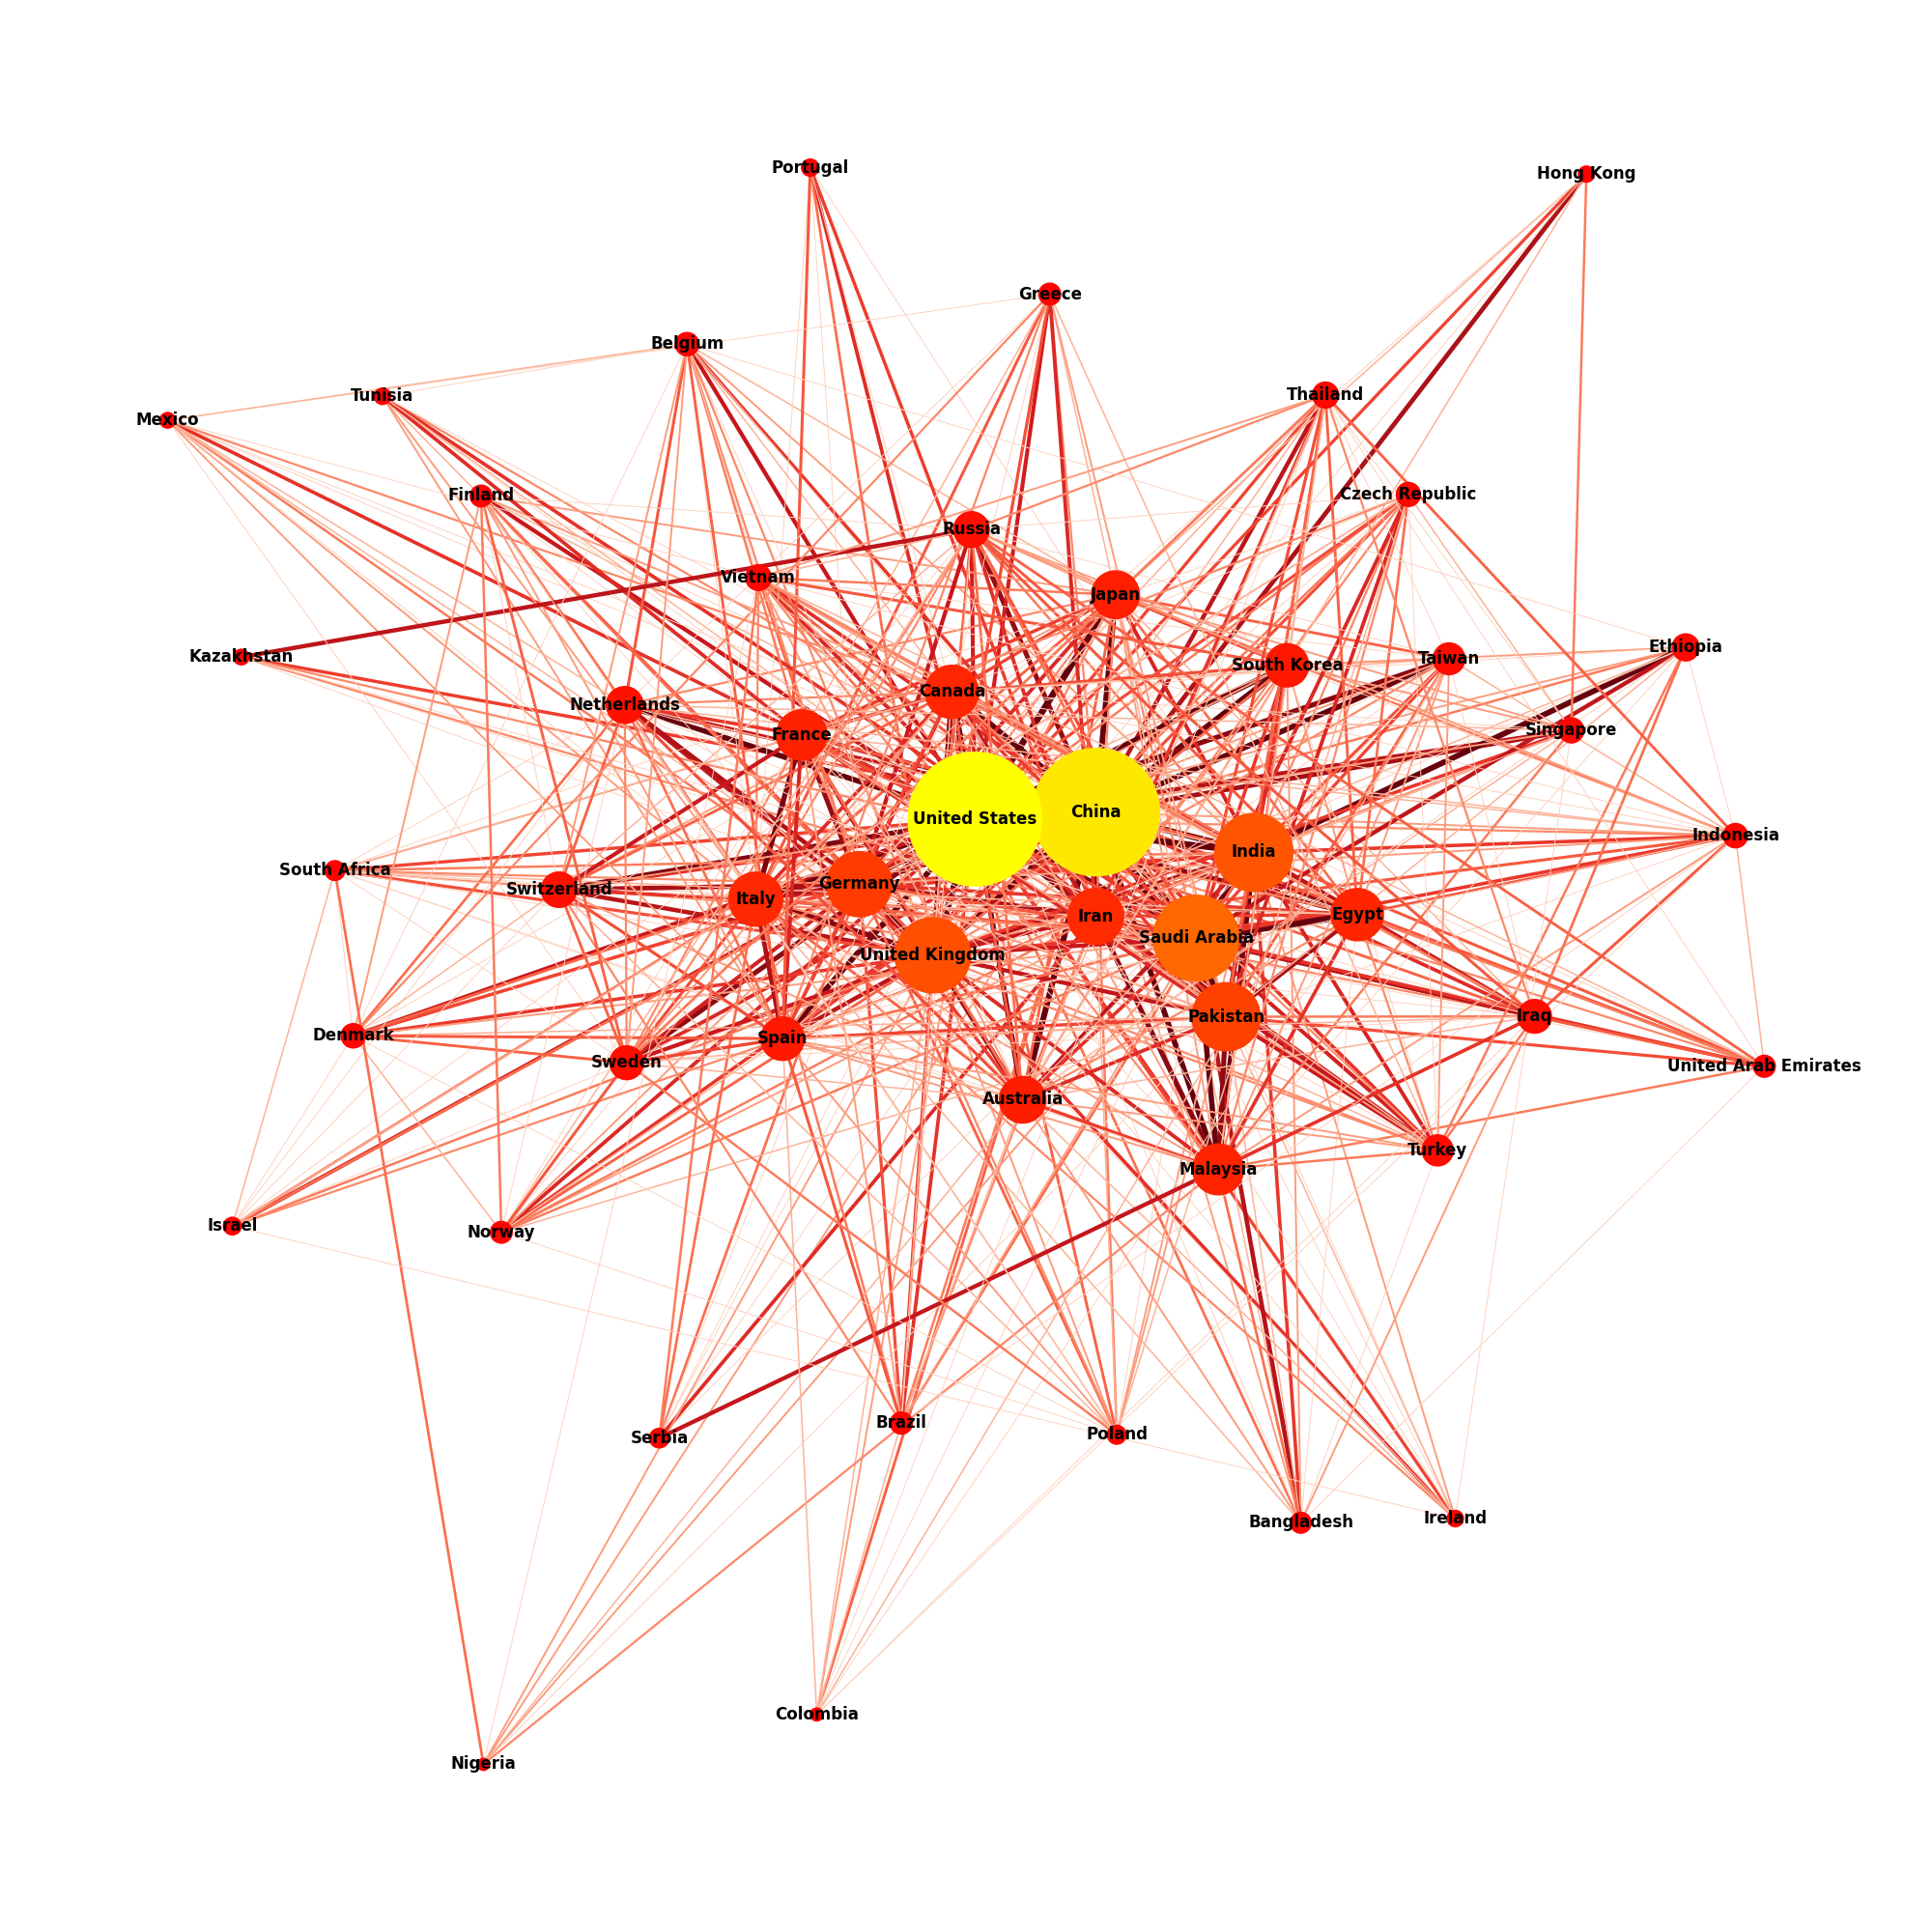
\includegraphics[width=0.8\textwidth]{network_graph_Country.png}
    \caption{Network Graph for Countries}
    \label{fig:country_network}
\end{figure}

Figure \ref{fig:country_network} shows the network of co-occurring countries in retraction cases with node sizes representing the frequency of retractions involving each country and edge thickness indicating the strength of collaboration or co-occurrence between countries. The weighted degree of each node highlights the centrality of certain countries within the network. Key observations include China and the United States as the most central nodes with weighted degrees of 2,086 and 2,238 respectively reflecting their high involvement in retraction cases and large research output. Saudi Arabia (1,107 weighted degree) and India (979 weighted degree) also show significant connections indicating their active roles in international collaborations and the occurrence of retractions. Other notable countries include the United Kingdom (901 weighted degree), Pakistan (759 weighted degree), and Germany (719 weighted degree) highlighting their involvement in the global research landscape. The dense network structure around central nodes shows extensive international collaborations leading to retractions implying that research integrity issues in one country can have far-reaching impacts.

\section{Distribution Analysis Based on Histogram Boxplot and Summary Statistics}
\begin{figure}[h!]
    \centering
    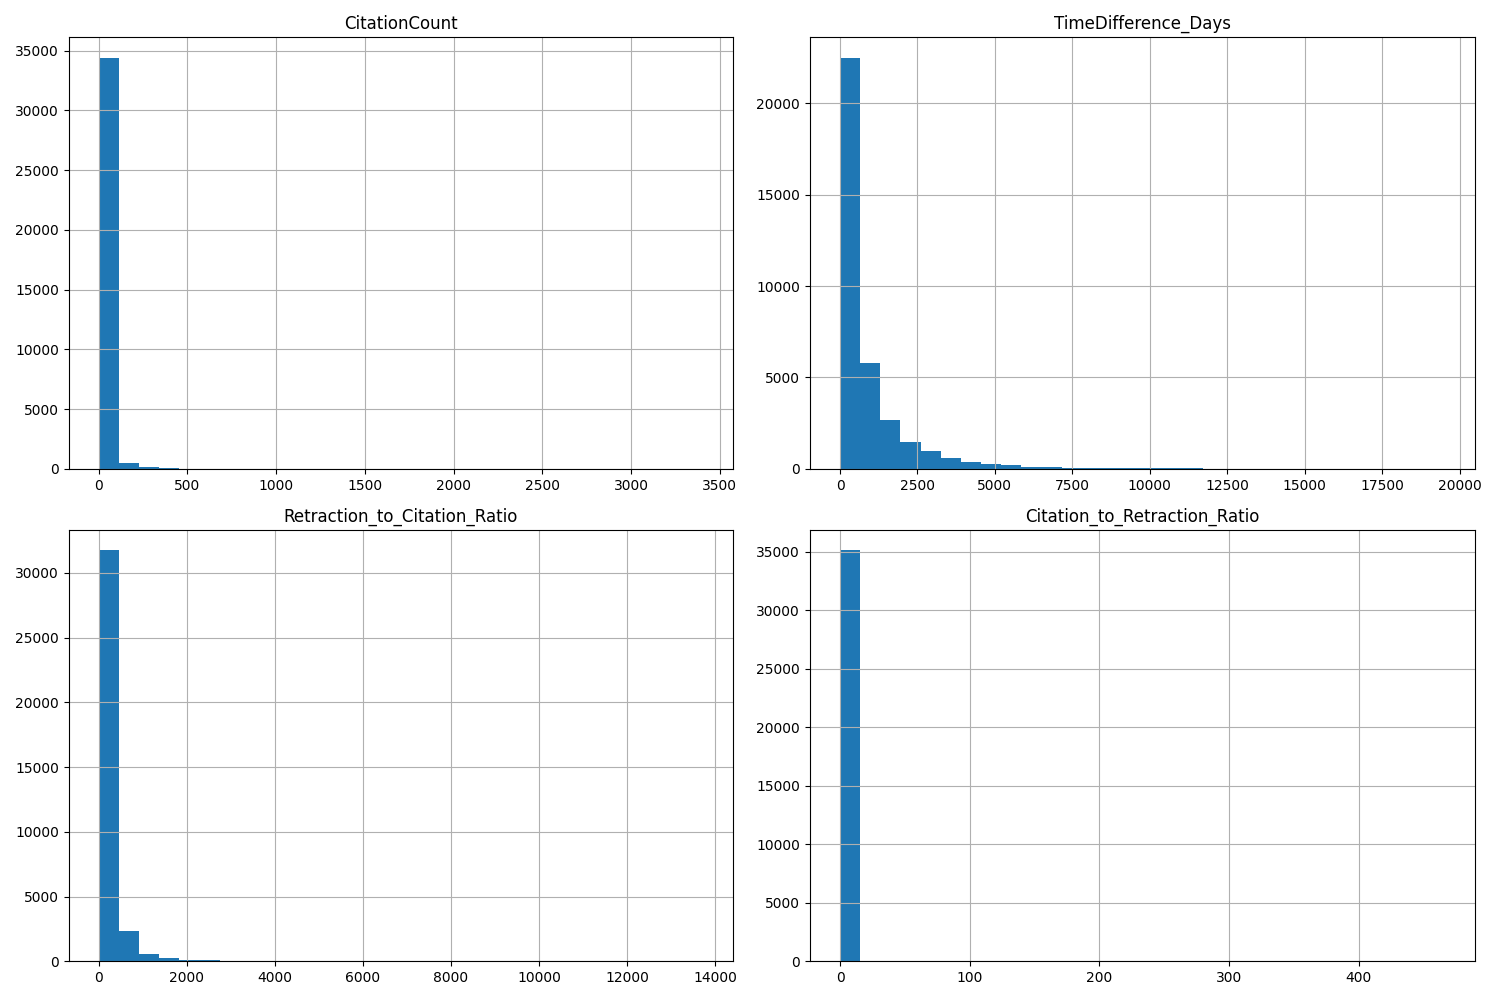
\includegraphics[width=1\textwidth]{distribution_analysis.png}
    \caption{Histogram analysis of numerical columns.}
    \label{fig:histogram}
\end{figure}
The distribution analysis of the retraction dataset as visualized through histograms, boxplots, and summary statistics reveals significant insights into the patterns and variability of key metrics. The histograms for metrics such as Retraction to Citation Ratio and Citation to Retraction Ratio show right-skewed distributions. This skewness is evident from the long tails extending towards higher values indicating that while most papers have lower ratios, a few papers with exceptionally high ratios skew the distribution. For instance, the Retraction to Citation Ratio has a mean of 193.23 much higher than the median of 69.10 reflecting the impact of outliers on the average. Similarly, the Citation to Retraction Ratio's mean of 0.21 is substantially higher than the median of 0.014 further illustrating the presence of a few highly cited retracted papers.

\begin{figure}[h!]
    \centering
    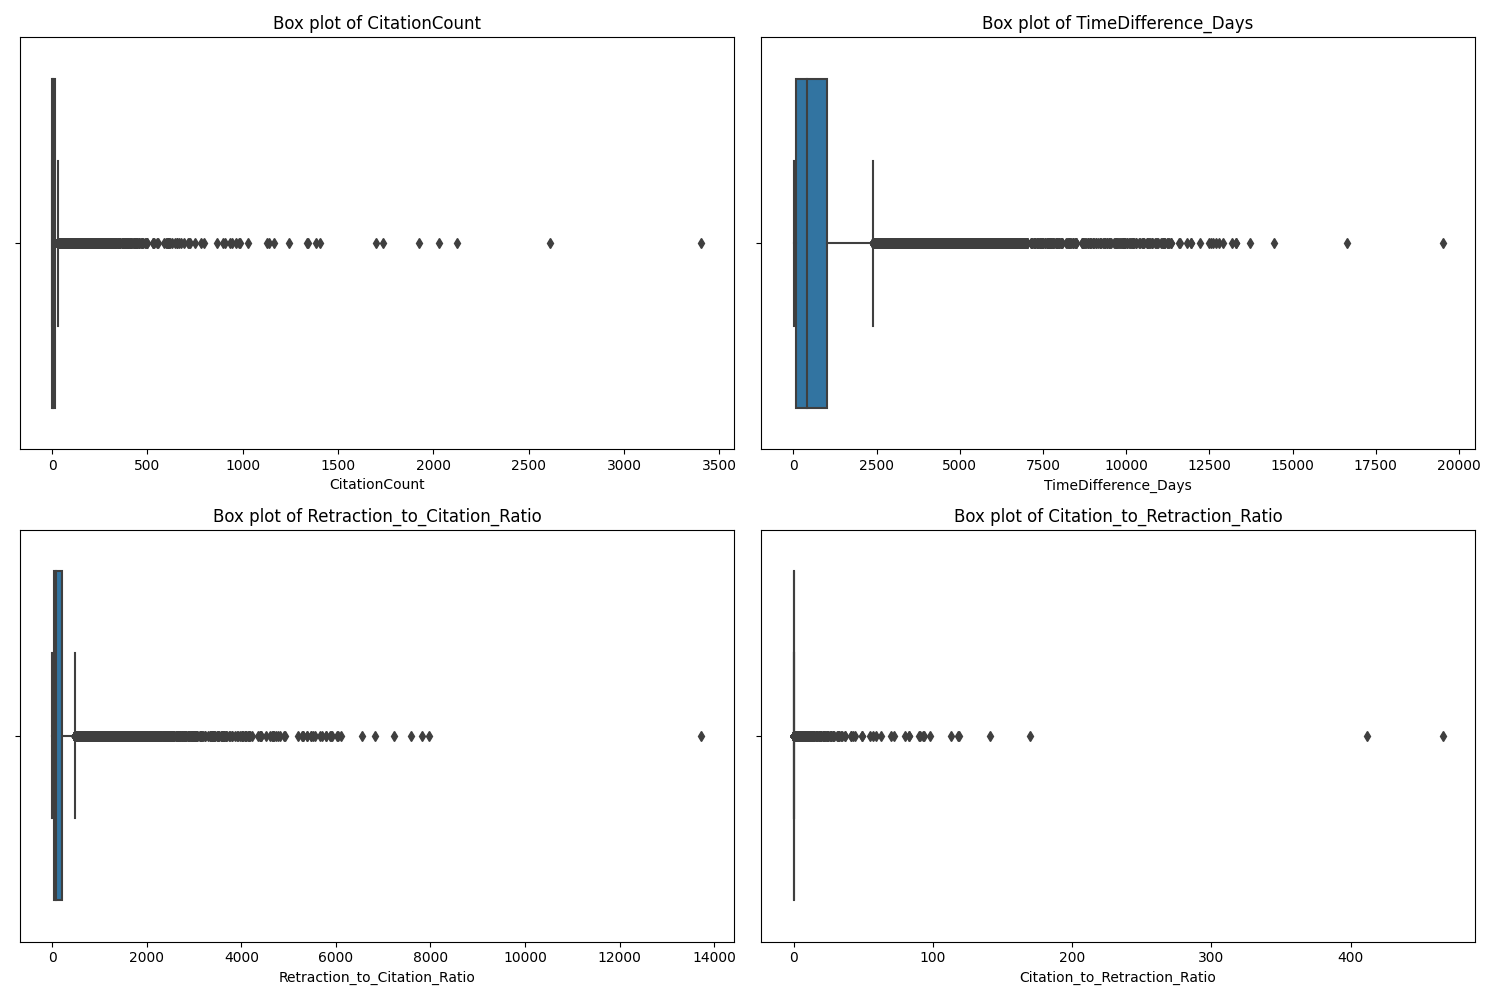
\includegraphics[width=1\textwidth]{box_plots.png}
    \caption{Boxplot analysis of numerical columns.}
    \label{fig:boxplot}
\end{figure} 
The boxplots complement this by highlighting the central tendency and spread of the data with the interquartile range (IQR) providing a clear view of the middle 50\% of the data. All box plots demonstrate extreme outliers which are crucial for understanding the complete distribution. For example, the Citation Count's boxplot shows a median of 2 indicating that half of the retracted papers have very few citations. However, the mean value of 15.93 and the presence of outliers as indicated by the maximum value of 3,406 suggest a right-skewed distribution. Similarly, the Time Difference in Days has a median of 393 days but a mean of 839.63 days with a maximum value of 19,511 days indicating a few papers that took exceptionally long to retract. These outliers while extreme provide important insights into the diverse nature of retraction cases and the variability in how long it takes for a paper to be retracted.

The summary statistics reinforce these observations by quantifying the central tendencies and variability. High standard deviations across all metrics such as 387.15 for Retraction to Citation Ratio and 4.19 for Citation to Retraction Ratio indicate considerable variability and the influence of outliers. These analyses collectively underscore the importance of addressing outliers and skewness in retraction data emphasizing the need for effective retraction processes to handle both typical and exceptional cases of research retraction.

\section{Correlation Matrix}

\begin{figure}[h!]
    \centering
    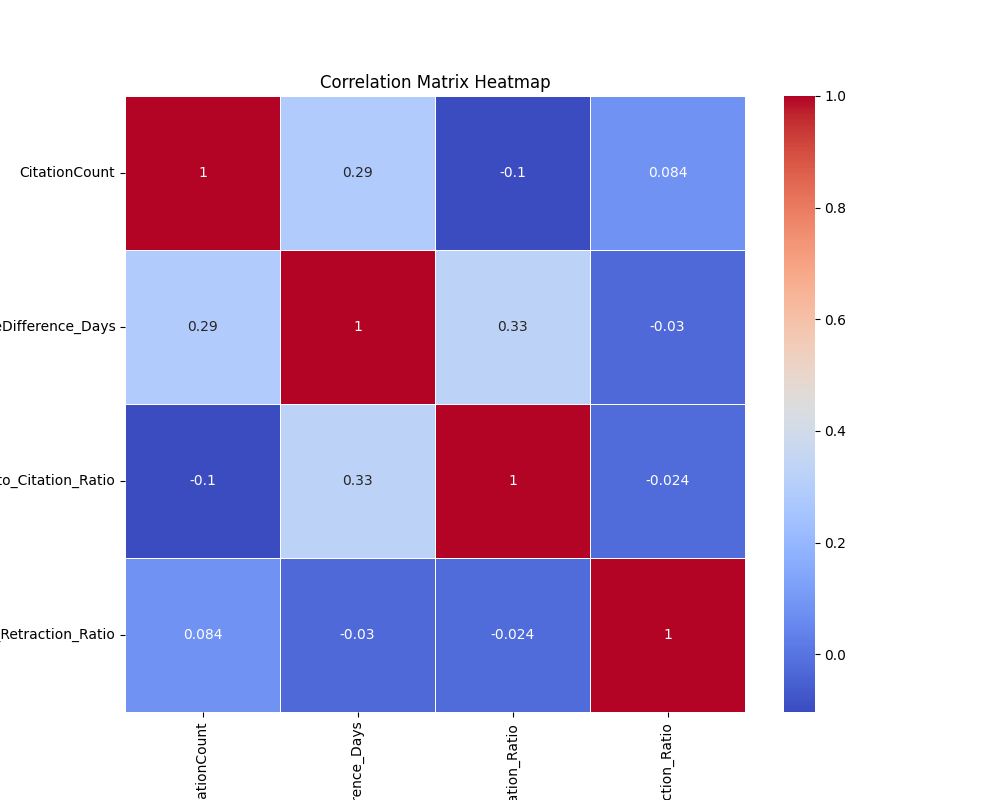
\includegraphics[width=0.8\textwidth]{correlation_matrix_heatmap.png}
    \caption{Correlation Matrix}
    \label{fig:correlation_matrix}
\end{figure}



\section{Time Series Analysis: Retraction and Publication}
The time series analysis highlights the dynamic nature of academic publishing and the increasing focus on research integrity. The parallel rise in retractions and publications underscores the importance of maintaining rigorous standards and oversight in the face of expanding research output. Understanding these trends helps in formulating strategies to address research misconduct and improve the overall quality of scientific literature.


\begin{figure}[h!]
    \centering
    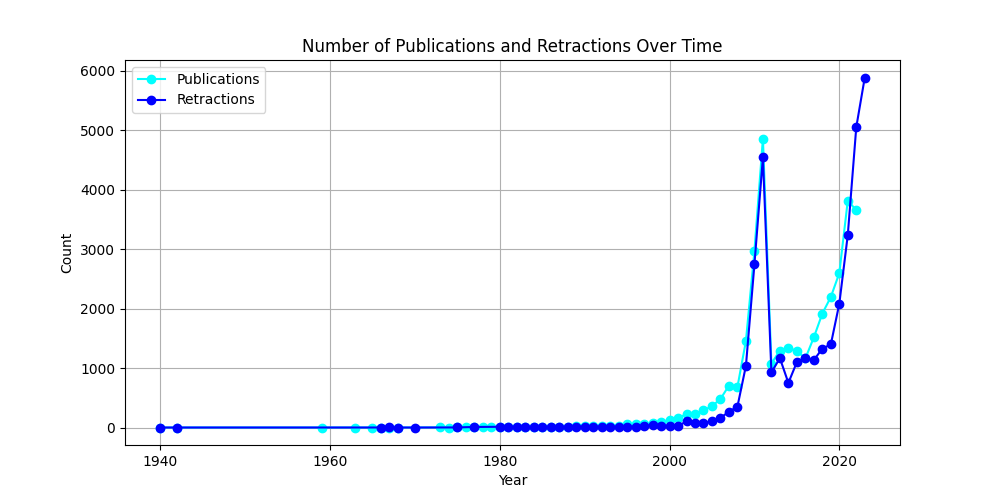
\includegraphics[width=0.8\textwidth]{publications_retractions_over_time.png}
    \caption{Publication and Retractions over time}
    \label{fig:publications_retractions_over_time}
\end{figure}


\begin{figure}[h!]
    \centering
    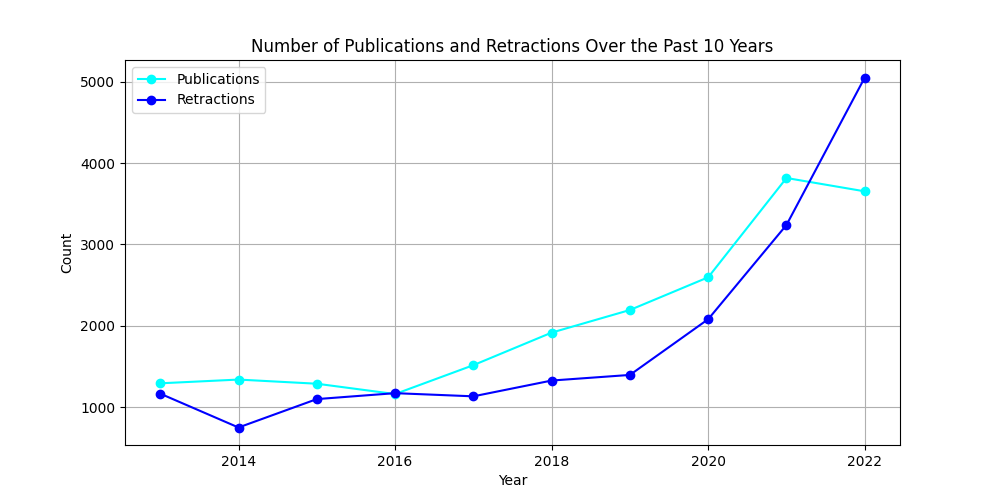
\includegraphics[width=0.8\textwidth]{publications_retractions_recent_years.png}
    \caption{Publication and Retractions in recent years.}
    \label{fig:publications_retractions_recent_years}
\end{figure}


\begin{table}[t!]
\centering
\caption{Key Observation}
\begin{tabular}{|p{7cm}|p{7cm}|}
\hline
\textbf{Retractions by Year} & \textbf{Publications by Year} \\
\hline
Retractions were relatively rare before the 1990s, with only a handful of cases each year. & Similar to retractions, the number of publications was relatively low before the 1990s. \\
\hline
Starting around 2002, there is a significant increase in the number of retractions, peaking in recent years. & There is a steady increase in the number of publications from the early 2000s, peaking in 2011 with 4,857 publications. \\
\hline
The number of retractions jumps sharply in 2009, reaching a peak in 2011 with 4,541 retractions. & The trend remains high with fluctuations, reaching another peak in 2021 with 3,817 publications. \\
\hline
After a brief dip in 2012, the trend continues to rise, with substantial increases in 2020 (2,082 retractions), 2021 (3,240 retractions), 2022 (5,052 retractions), and reaching the highest in 2023 with 5,886 retractions. & The recent years (2020-2022) show a significant volume of publications, although slightly lower than the peak in 2011. \\
\hline
This upward trend could be attributed to several factors, including increased scrutiny of published research, the proliferation of predatory journals, and the rise of digital tools for detecting research misconduct. & The increase in publications likely reflects the growth of global research activity, advances in technology, and the expansion of academic publishing. \\
\hline
\end{tabular}
\end{table}
\clearpage
\newpage
\subsection{Retractions Over Time for Top 5 Subjects}
\begin{figure}[t]
\centering
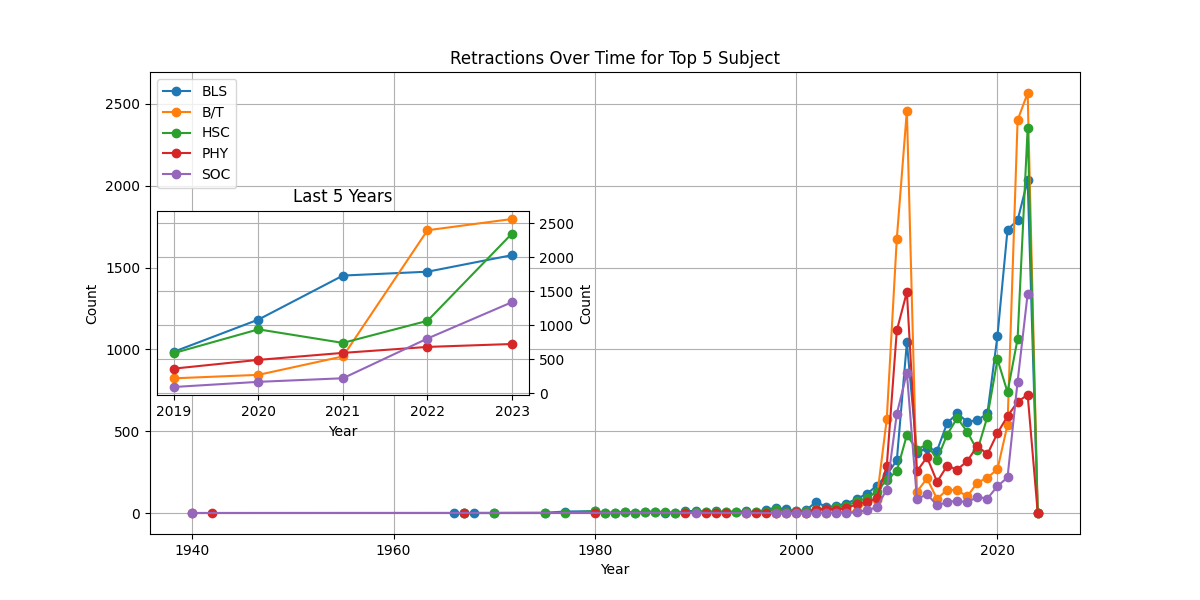
\includegraphics[width=0.8\textwidth]{time_series_Subject.png}
\caption{Retractions Over Time for Top 5 Subjects}
\label{fig
}
\end{figure}

Figure \ref{fig
} shows the trends in retractions over time for the top 5 subjects: BLS, B/T, HSC, PHY, and SOC. The long-term trend reveals that all five subjects experienced a significant increase in retractions starting around 2010 peaking in 2011 and again in recent years. This indicates a heightened level of scrutiny and possibly more rigorous retraction practices in these fields over the past decade. The inset for the last five years highlights a steady increase in retractions from 2019 to 2023 with B/T and BLS showing the highest counts in 2023. This recent trend reflects ongoing issues and increased vigilance in these academic disciplines. This upward trend could be attributed to several factors including increased scrutiny of published research, the proliferation of predatory journals, and the rise of digital tools for detecting research misconduct.

\subsection{Retractions Over Time for Top 5 Journals}
\begin{figure}[h!]
\centering
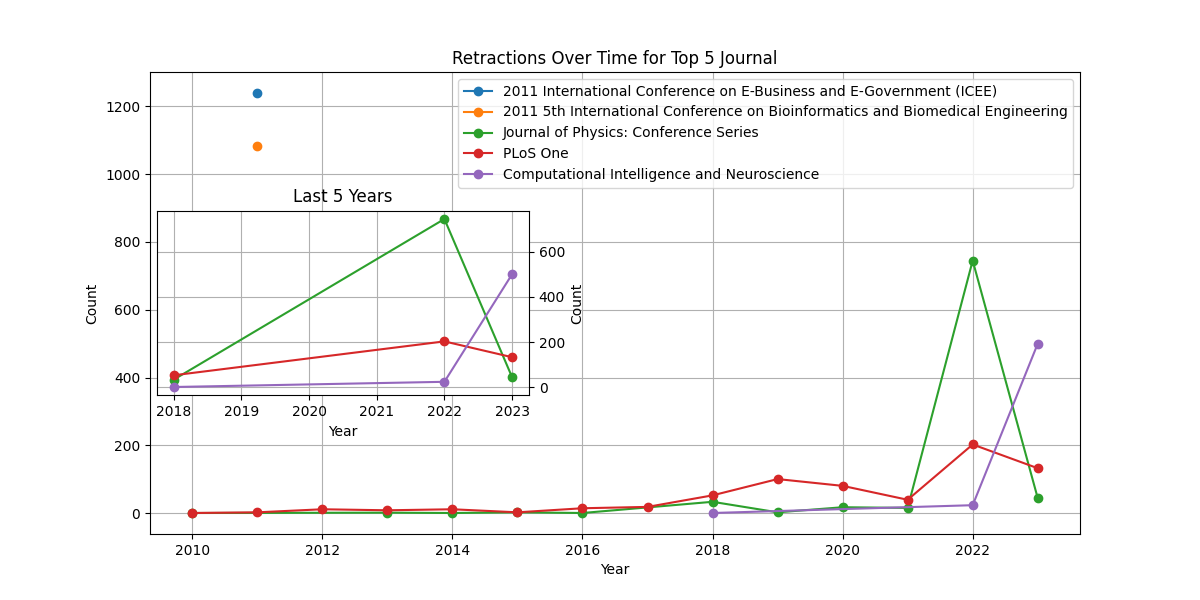
\includegraphics[width=0.8\textwidth]{time_series_Journal.png}
\caption{Retractions Over Time for Top 5 Journals}
\label{fig
}
\end{figure}

Figure \ref{fig
} illustrates the trends in retractions over time for the top 5 journals. The long-term trend shows spikes in retractions for "2011 International Conference on E-Business and E-Government (ICEE)" and "2011 5th International Conference on Bioinformatics and Biomedical Engineering" around 2011 indicating specific issues during that period. There is also a significant increase in retractions for "Journal of Physics: Conference Series" around 2022. The inset for the last five years reveals a sharp rise in retractions for "Journal of Physics: Conference Series" in 2022 while other journals show fluctuations highlighting ongoing problems and the impact of enhanced detection methods.

\subsection{Retractions Over Time for Top 5 Authors}
\begin{figure}[h!]
\centering
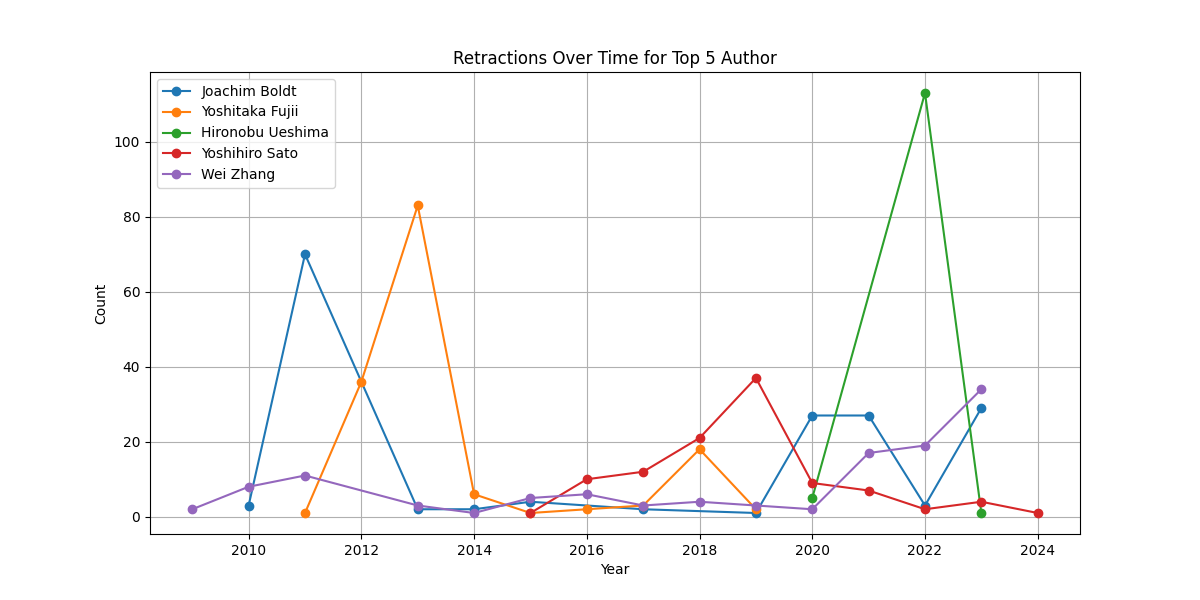
\includegraphics[width=0.8\textwidth]{time_series_Author.png}
\caption{Retractions Over Time for Top 5 Authors}
\label{fig
}
\end{figure}

Figure \ref{fig
} tracks the trends in retractions for the top 5 authors. The long-term trend shows noticeable spikes for Joachim Boldt around 2011 and Yoshitaka Fujii around 2012 indicating periods of intense scrutiny and numerous retractions for these authors. In the last five years the inset reveals a significant increase in retractions for Wei Zhang and Hironobu Ueshima around 2022 suggesting recent issues with their publications and possible investigations leading to these retractions.

\subsection{Retractions Over Time for Top 5 Publishers}
\begin{figure}[t]
\centering
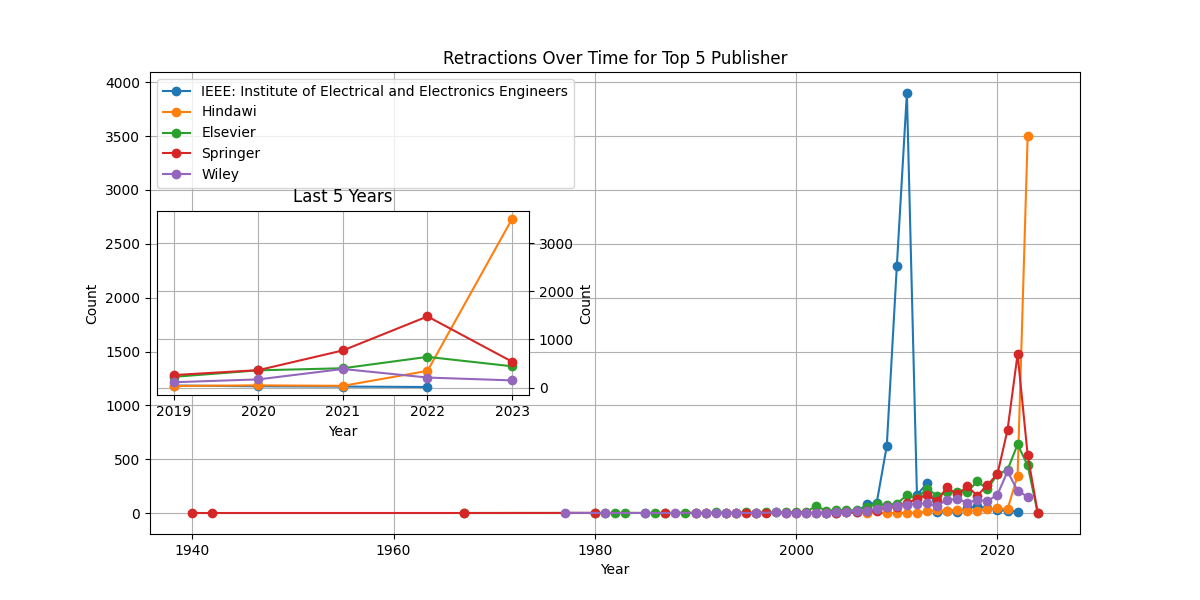
\includegraphics[width=0.8\textwidth]{time_series_Publisher.png}
\caption{Retractions Over Time for Top 5 Publishers}
\label{fig
}
\end{figure}

Figure \ref{fig
} presents the trends in retractions over time for the top 5 publishers: IEEE, Hindawi, Elsevier, Springer, and Wiley. The long-term trend indicates that IEEE and Hindawi experienced significant spikes in retractions around 2011 and in recent years. This pattern suggests periods of increased retractions possibly due to more rigorous editorial standards or higher detection rates of problematic papers. The inset for the last five years highlights substantial increases in retractions for Hindawi in 2023 reflecting ongoing issues and the impact of increased scrutiny on their publications.

\subsection{Retractions Over Time for Top 5 Countries}
\begin{figure}[t]
\centering
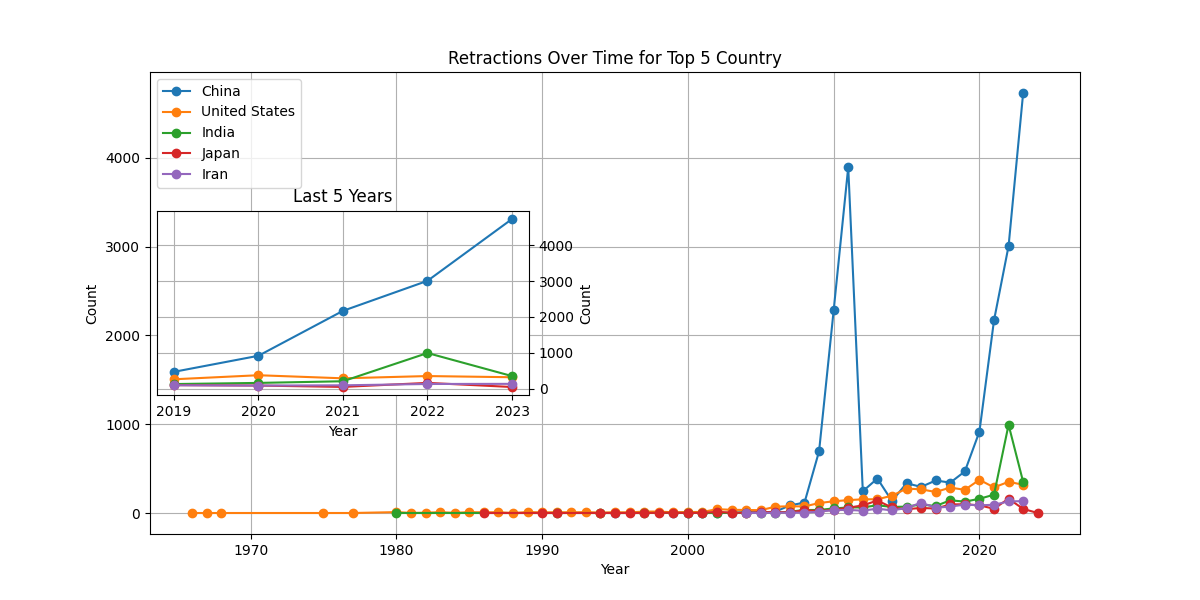
\includegraphics[width=0.8\textwidth]{time_series_Country.png}
\caption{Retractions Over Time for Top 5 Countries}
\label{fig
}
\end{figure}

Figure \ref{fig
} shows the trends in retractions over time for the top 5 countries: China, United States, India, Japan, and Iran. The long-term trend reveals that China and the United States have the highest retraction counts with notable spikes around 2010 and 2023 for China. This indicates significant periods of increased retractions for these countries possibly due to heightened scrutiny and improved detection mechanisms. The inset for the last five years shows a consistent rise in retractions for China from 2019 to 2023 reflecting ongoing challenges and increased vigilance within the country.

\subsection{Retractions Over Time for Top 5 Article Types}
\begin{figure}[t]
\centering
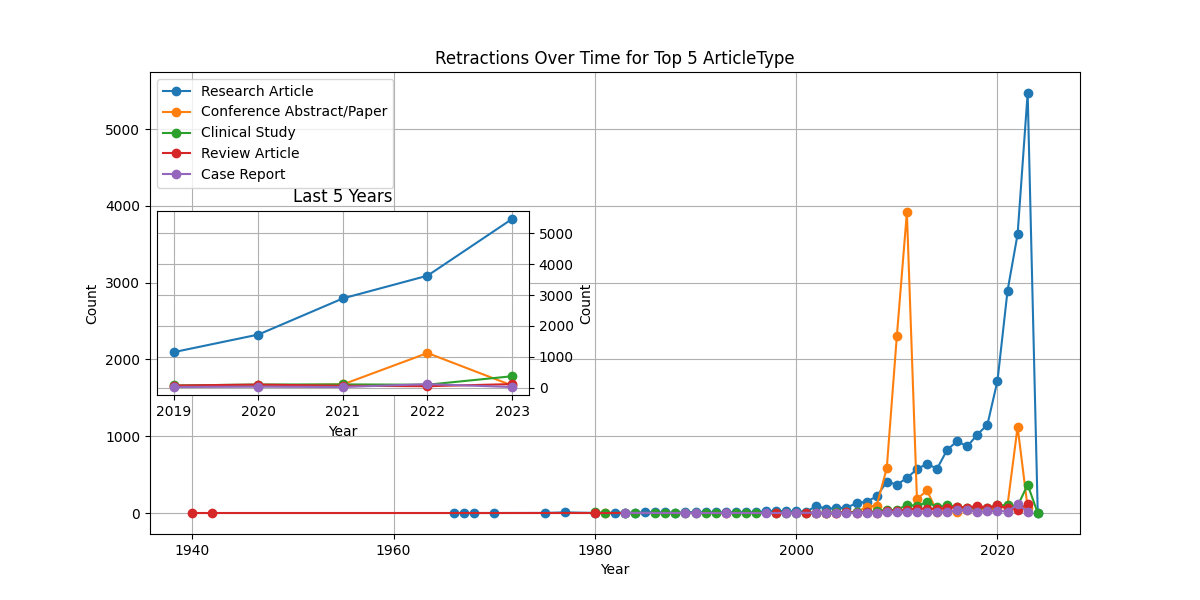
\includegraphics[width=0.8\textwidth]{time_series_ArticleType.png}
\caption{Retractions Over Time for Top 5 Article Types}
\label{fig
}
\end{figure}

Figure \ref{fig
} illustrates the trends in retractions over time for the top 5 article types: Research Article, Conference Abstract/Paper, Clinical Study, Review Article, and Case Report. The long-term trend shows that research articles have the highest number of retractions with significant increases around 2010 and in recent years. This pattern indicates that research articles are particularly prone to retractions possibly due to their higher volume and impact. The inset for the last five years highlights a steady increase in retractions for research articles and conference papers reflecting ongoing issues with these publication types and the effect of enhanced retraction practices.

\subsection{Retractions Over Time for Top 5 Reasons}
\begin{figure}[h!]
\centering
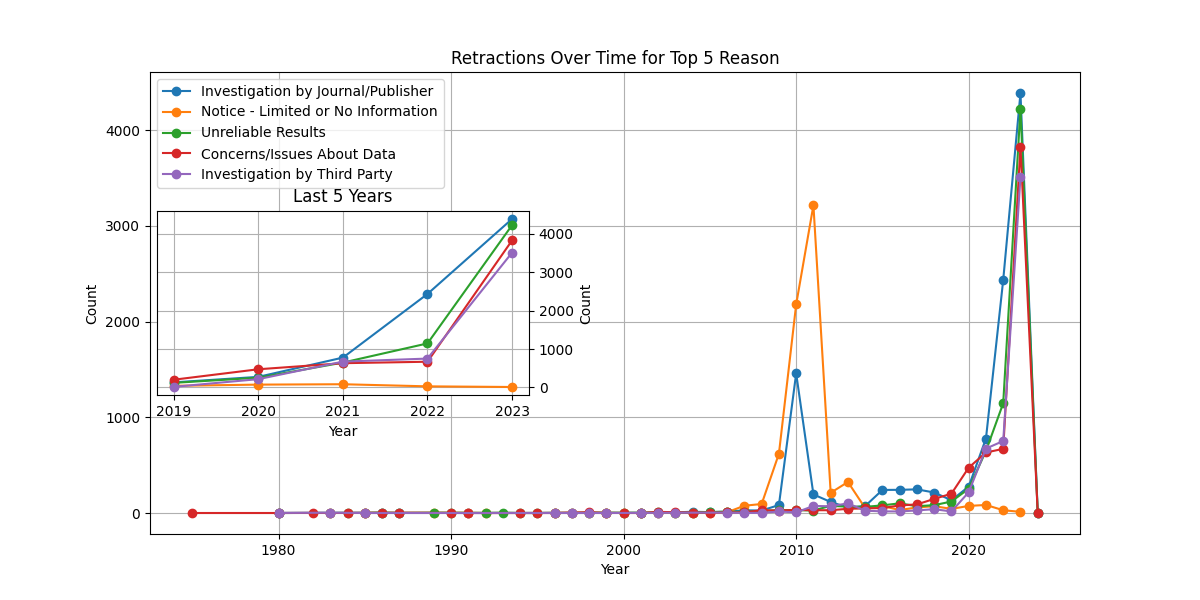
\includegraphics[width=0.8\textwidth]{time_series_Reason.png}
\caption{Retractions Over Time for Top 5 Reasons}
\label{fig
}
\end{figure}

Figure \ref{fig
} tracks the trends in retractions over time for the top 5 retraction reasons: +Investigation by Journal/Publisher, +Notice - Limited or No Information, +Unreliable Results, +Concerns/Issues About Data, and +Investigation by Third Party. The long-term trend reveals notable increases around 2010 and in recent years with investigations by journals/publishers and unreliable results being the most frequent reasons for retractions. The inset for the last five years shows significant increases in retractions for investigations by journals/publishers and concerns about data from 2019 to 2023 indicating that these remain major issues contributing to retractions.

\section{Key Points}
The analysis of retractions and citations reveals significant patterns across various categories. Among subjects, Biological Sciences (BLS) and Biotechnology/Technical Sciences (B/T) lead with the highest number of retractions (12,679 and 11,337 respectively) while Biological Sciences also have the highest citation count (347,126). Journals such as "2011 5th International Conference on Bioinformatics and Biomedical Engineering" and "PLoS One" show notable retraction counts with the latter also having a high citation count (17,832.9). Among publishers, IEEE leads with 7,135 retractions while Elsevier has the highest citation count (115,214.2). Country-wise, China tops the retraction list with 19,738 cases while the United States has the highest citation count (178,226.9). Research Articles are the most retracted article type (21,903) and also have the highest citation count (439,408.0). Regarding reasons for retraction, "Investigation by Journal/Publisher" accounts for the highest number of retractions (10,818) while "Concerns/Issues About Data" has the highest citation count (106,369.4). These insights underscore the widespread nature of retractions across disciplines, journals, publishers, countries, article types, and retraction reasons highlighting the complex landscape of research integrity.

\begin{figure}[t]
    \centering
    \begin{minipage}[b]{0.48\textwidth}
        \centering
        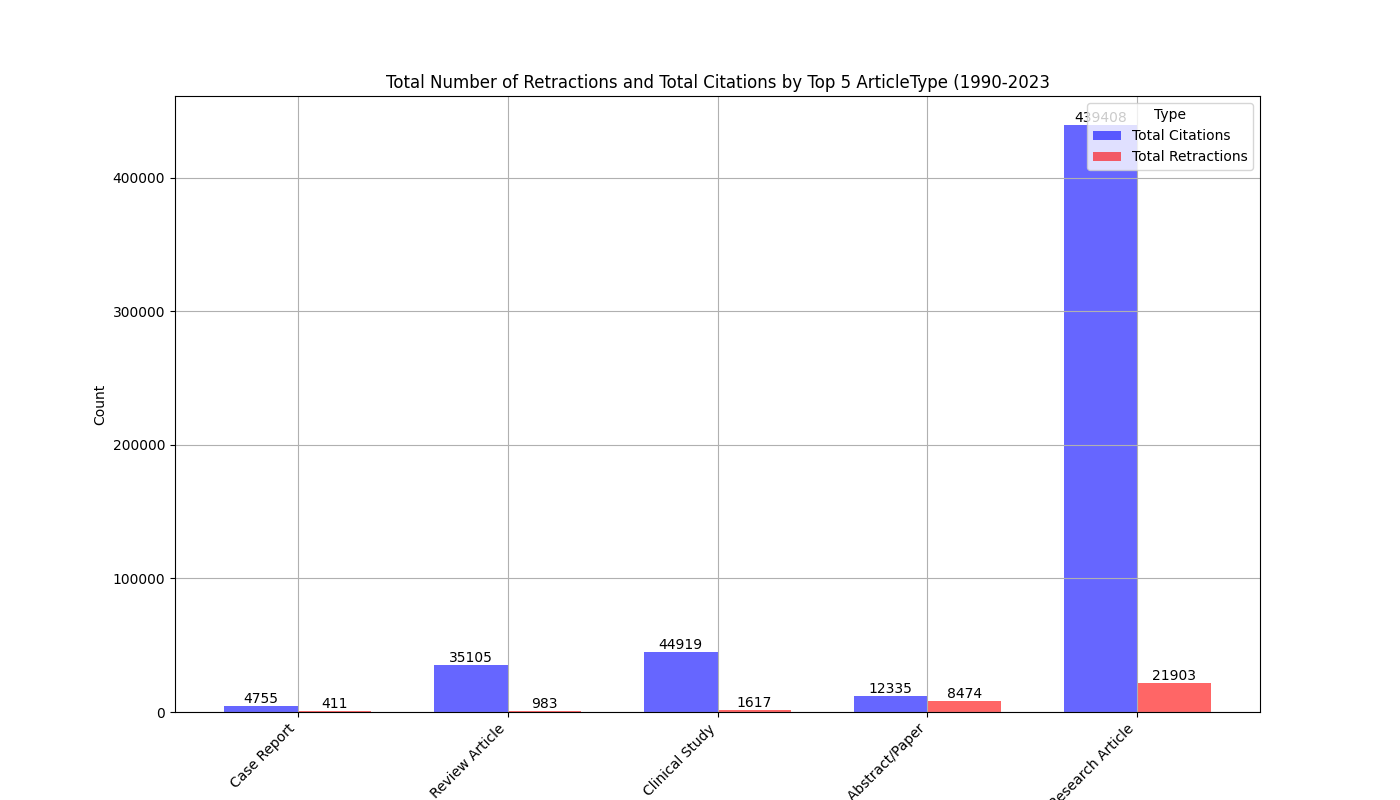
\includegraphics[width=\textwidth]{retractions_and_citations_ArticleType.png}
        \caption{Retractions and Citations by Article Type}
        \label{fig:ArticleType}
    \end{minipage}
    \hfill
    \begin{minipage}[b]{0.48\textwidth}
        \centering
        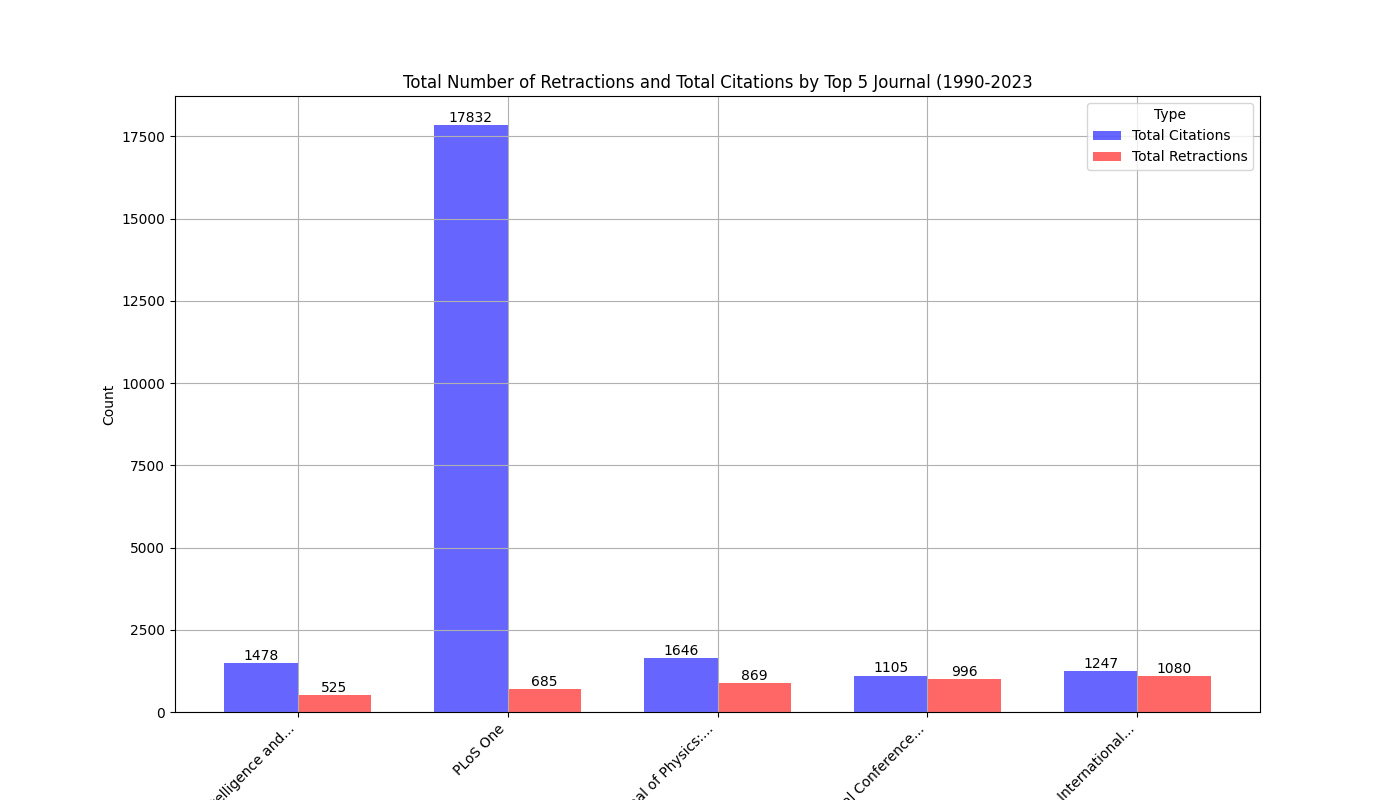
\includegraphics[width=\textwidth]{retractions_and_citations_Journal.png}
        \caption{Retractions and Citations by Journal}
        \label{fig:Journal}
    \end{minipage}
    \vfill
    \begin{minipage}[b]{0.48\textwidth}
        \centering
        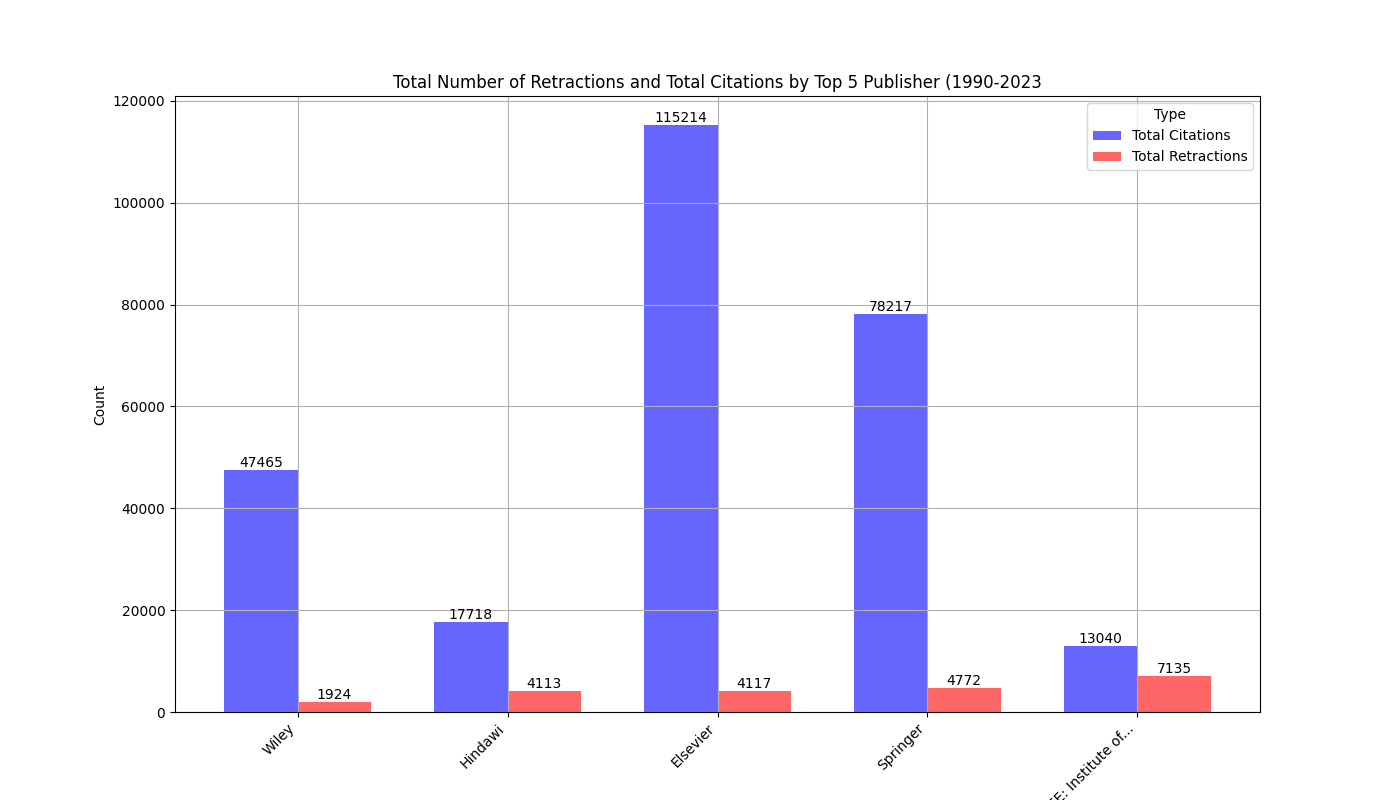
\includegraphics[width=\textwidth]{retractions_and_citations_Publisher.png}
        \caption{Retractions and Citations by Publisher}
        \label{fig:Publisher}
    \end{minipage}
    \hfill
    \begin{minipage}[b]{0.48\textwidth}
        \centering
        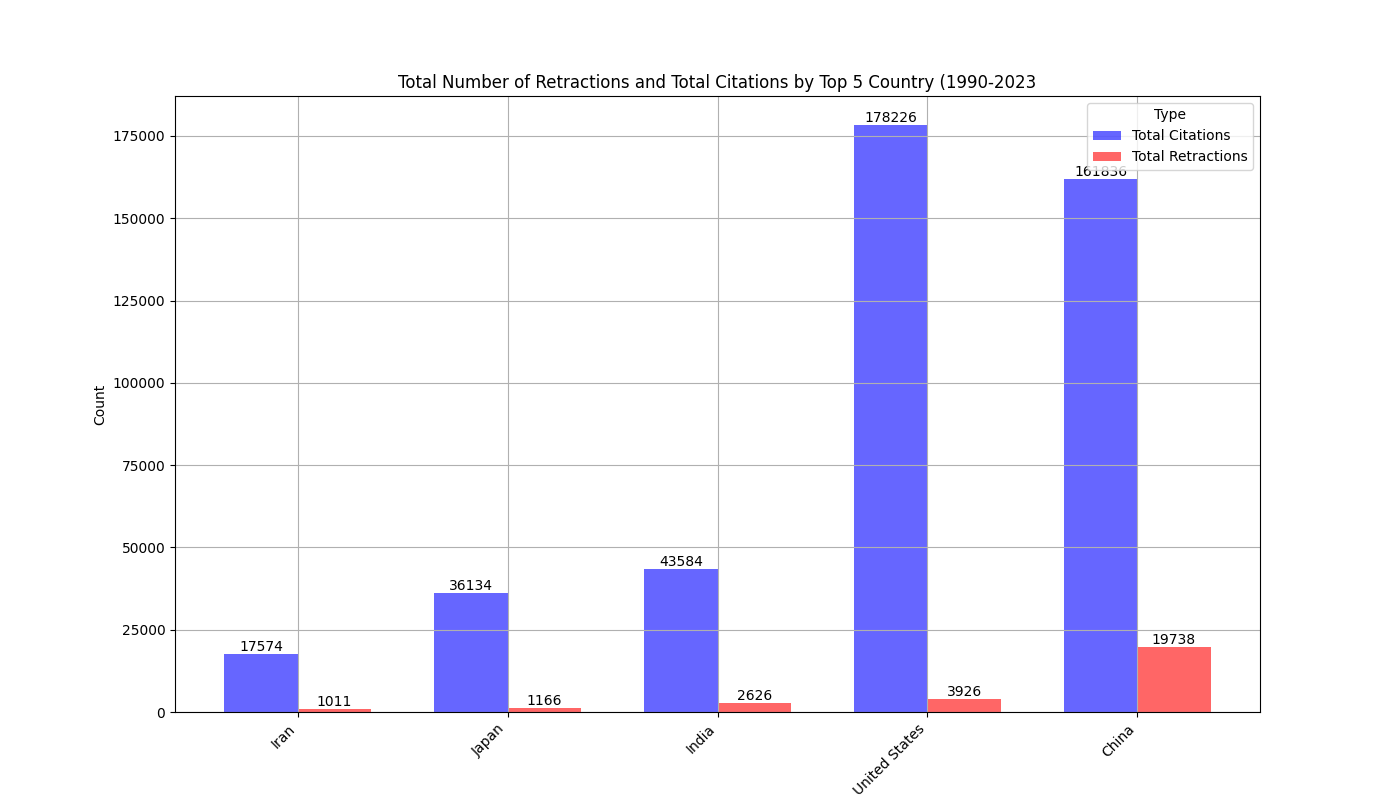
\includegraphics[width=\textwidth]{retractions_and_citations_Country.png}
        \caption{Retractions and Citations by Country}
        \label{fig:Country}
    \end{minipage}
    \vfill
    \begin{minipage}[b]{0.48\textwidth}
        \centering
        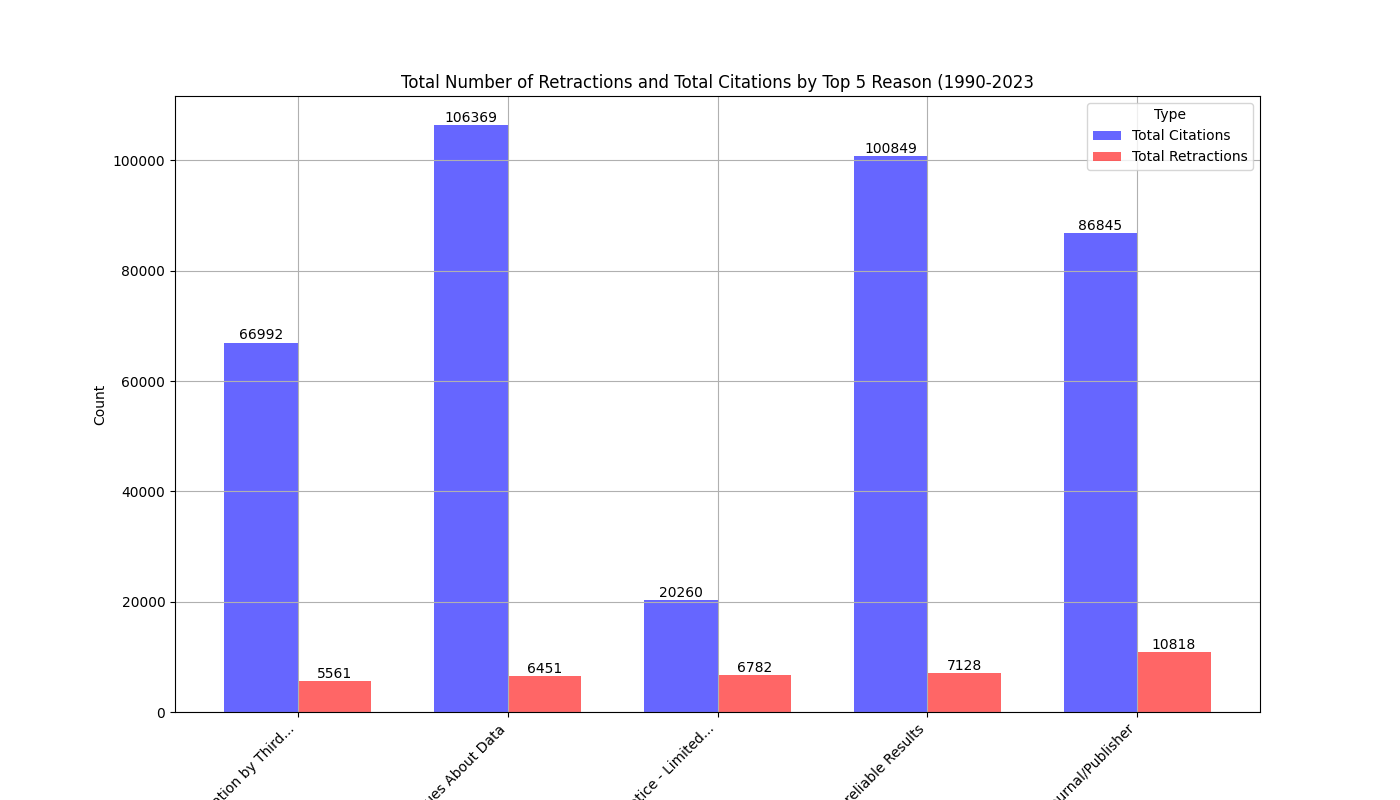
\includegraphics[width=\textwidth]{retractions_and_citations_Reason.png}
        \caption{Retractions and Citations by Reason}
        \label{fig:Reason}
    \end{minipage}
    \hfill
    \begin{minipage}[b]{0.48\textwidth}
        \centering
        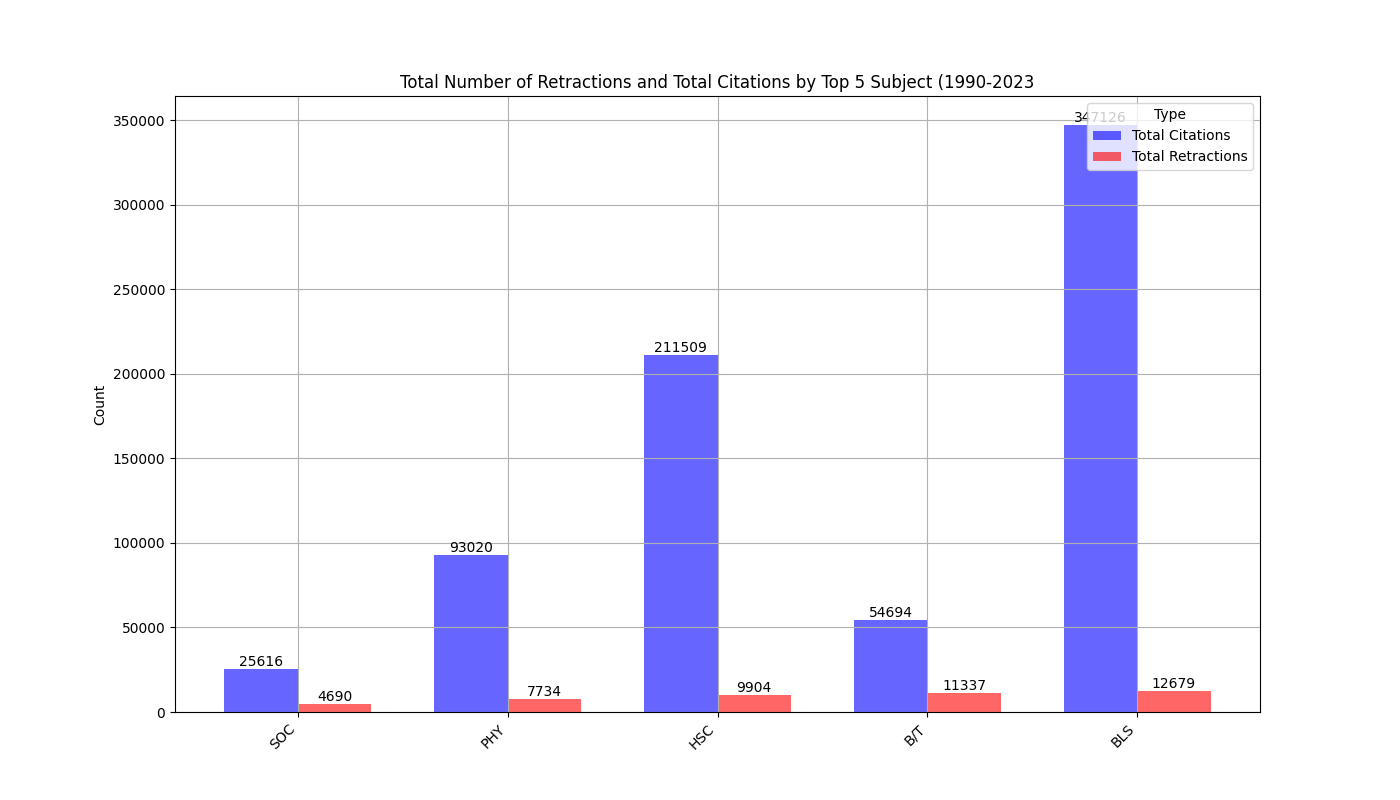
\includegraphics[width=\textwidth]{retractions_and_citations_Subject.png}
        \caption{Retractions and Citations by Subject}
        \label{fig:Subject}
    \end{minipage}
    \caption{Retractions and Citations Analysis}
    \label{fig:retractions_and_citations}
\end{figure}

\section{Predictive Modeling: Approach 1}
\subsection{Data Preprocessing and Outlier Handling}
\begin{itemize}
    \item \textbf{Convert to Numeric:}
    \begin{itemize}
        \item The categorical columns whose value is a string are converted to numeric by factorizing them. This is essential for numerical modeling since most machine learning algorithms cannot handle categorical data directly.
        \item Dropping missing values ensures the dataset is clean, but it can also lead to the loss of data.
    \end{itemize}
    
    \item \textbf{Null Value Check:}
    \begin{itemize}
        \item Before handling outliers, it is crucial to check for null values in the dataset. This step ensures that any missing values are identified and appropriately managed, either by imputation or removal.
        \item Handling null values ensures the integrity of the dataset and prevents errors during the modeling process.
    \end{itemize}
    
    \item \textbf{Handle Outliers:}
    \begin{itemize}
        \item Identify outliers using z-scores, considering data points with z-scores beyond $\pm 3$ as outliers.
        \item Outliers are replaced with NaN and then imputed with the median of the column. This helps in reducing the impact of extreme values without completely removing data points.
    \end{itemize}
    
    \item \textbf{Creating a New DataFrame for Analysis:}
    \begin{itemize}
        \item The new dataframe is prepared for analysis focusing on retraction reasons, their frequency, and mean duration between publication and retraction. This involves ensuring the 'Reason' column is string-type, splitting it into individual reasons, removing leading and trailing whitespace, and aggregating data by 'Reason' to derive valuable insights.
    \end{itemize}
\end{itemize}


\subsection*{Base Model}
The baseline model provides a benchmark for comparison and reveals the magnitude of improvement achievable with more sophisticated models.


\begin{figure}[h!]
\centering
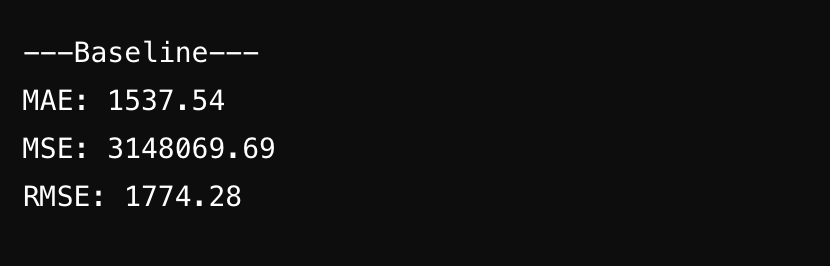
\includegraphics[width=0.8\textwidth]{baseline_model_output.png}
\caption{Baseline Model Output}
\label{fig
}
\end{figure}

\begin{itemize}
    \item \textbf{Mean Absolute Error (MAE):} The baseline MAE of 1537.54 indicates that, on average, the baseline model's predictions are off by approximately 1538 days from the actual values. This suggests that the baseline model is not accurate in predicting the retraction duration.
    \item \textbf{Mean Squared Error (MSE):} The baseline MSE of 3148069.69 indicates large errors in some predictions. Since MSE squares the errors, it penalizes larger errors more heavily than MAE.
    \item \textbf{Root Mean Squared Error (RMSE):} The baseline RMSE of 1774.28 is the square root of MSE, providing the error in the same units as the target variable. Despite the low number, it seems suspiciously small compared to the range of target values, indicating potential issues with the model's performance.
\end{itemize}

\subsection*{Random Forest Regressor}


\begin{figure}[h!]
\centering
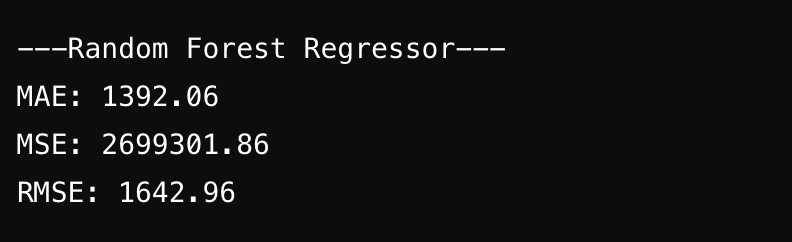
\includegraphics[width=0.8\textwidth]{random_forest_output.png}
\caption{Random Forest Regressor Output}
\label{fig
}
\end{figure}

\begin{itemize}
    \item \textbf{Mean Absolute Error (MAE):} The MAE of 1392.06 suggests that, on average, the predictions of the random forest regressor model are off by approximately 1392 days from the actual values.
    \item \textbf{Mean Squared Error (MSE):} The MSE of 2699301.86 indicates large errors in some predictions, but it is lower compared to the baseline model.
    \item \textbf{Root Mean Squared Error (RMSE):} The RMSE of 1642.96 is lower than the baseline RMSE, indicating that the random forest regressor model performs better in terms of error compared to the baseline model.
\end{itemize}

\subsection*{Hyperparameter Tuning}
The hyperparameters identified for the tuned model (e.g., max depth, min samples leaf, \texttt{n\_estimators} are optimized for the dataset. These parameters were chosen through a process that aims to enhance the model's performance.

\begin{figure}[h!]
\centering
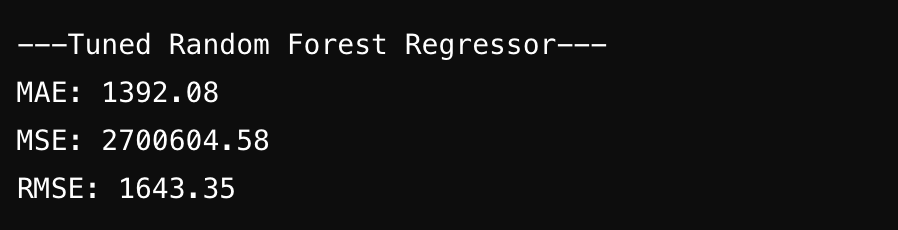
\includegraphics[width=0.8\textwidth]{random_forest_tuning_output.png}
\caption{Random Forest Regressor Output after Hyperparameter Tuning}
\label{fig
}
\end{figure}



\begin{itemize}
    \item \textbf{Mean Absolute Error (MAE):} The MAE of 1392.08 is very similar to that of the untuned random forest regressor model, suggesting that the tuning did not significantly improve the model's performance in terms of MAE.
    \item \textbf{Mean Squared Error (MSE):} The MSE of 2700604.58 is slightly higher than that of the untuned model, indicating slightly worse performance in terms of squared errors.
    \item \textbf{Root Mean Squared Error (RMSE):} The RMSE of 1643.35 is very close to that of the untuned model, indicating that the tuning did not substantially affect the model's performance in terms of RMSE.
\end{itemize}
In evaluating the predictive models for retraction duration it becomes evident that the Random Forest Regressor stands as a marked improvement over the baseline model. The baseline's notably high Mean Absolute Error (MAE) of 1537.54 days signifies its substantial inaccuracies in predicting retraction durations. Meanwhile, the Random Forest Regressor with its lower MAE of 1392.06 days demonstrates a tangible enhancement in predictive accuracy. This improvement is further corroborated by its lower Mean Squared Error (MSE) and Root Mean Squared Error (RMSE) indicating a reduction in both systematic and overall prediction errors compared to the baseline.

Hyperparameter tuning a technique aimed at refining model performance yielded limited benefits in this context. Despite efforts to optimize parameters such as max depth min samples leaf and \texttt{n\_estimators} the tuned Random Forest Regressor showcased only marginal improvements over its untuned counterpart. The similarity in MAE MSE and RMSE values between the tuned and untuned models suggests that the default hyperparameters may already be reasonably well-suited for the dataset. Alternatively it hints at the possibility that other hyperparameters not addressed in this tuning process could hold more significant sway over model performance.

While the Random Forest Regressor outshines the baseline model the quest for even greater predictive accuracy remains ongoing. Although hyperparameter tuning did not yield substantial enhancements in this instance it underscores the iterative nature of model refinement. Further exploration of hyperparameters or consideration of alternative models may hold promise for achieving heightened predictive precision. Additionally deeper investigation into the dataset's characteristics and potential feature engineering endeavors could unveil avenues for refining model performance beyond the scope of hyperparameter tuning alone.

\section{Predictive Modelling: Approach 2}
\subsection{Preprocessing}
In preparation for academic analysis the dataset underwent a cleaning process to ensure data integrity and focus on the most relevant information. Duplicate entries were removed to eliminate redundancy. Irrelevant columns containing details like "Author" "OriginalPaperDate" "RetractionNature" and "RetractionDate" were excluded to streamline the data and prioritize key variables.

Categorical variables were further refined by identifying and replacing inconsistent entries within cells with the most frequent value. This step helped reduce noise and maintain data accuracy. Finally the "Reason" column was cleaned by removing unnecessary characters improving readability for further analysis. These preprocessing steps were crucial in creating a well-structured and clean dataset providing a solid foundation for subsequent modeling endeavors.

\subsection{Selecting the Target Variables}
Selecting a target variable for our analysis presented several challenges. The primary difficulty was choosing a variable that encapsulated the core aspects of the analysis while aligning with our project's goals. Since the dataset focused on retractions in academic publications identifying a meaningful indicator of retraction severity or impact was crucial. Additionally ensuring the availability and reliability of data for the chosen target variable presented another hurdle.

Given the limitation that the "RetractionNature" column has only one value it offered minimal variation for modeling purposes. To address this constraint we opted for "TimeDifference Days" as the target feature.
\begin{itemize}
\item TimeDifference Days represents the number of days between a paper's publication and its retraction.
\item Analyzing this timing can help us uncover factors influencing retraction timelines ultimately contributing to improved academic practices.
\item With TimeDifference Days as the target variable we can potentially predict when future retractions might occur using straightforward regression techniques. It's important to remember however that such predictions are likely probabilistic and may not be foolproof.
\item By gaining insights into retraction timelines through TimeDifference Days we can take proactive steps to prevent potential retractions promoting integrity within scholarly research.
\end{itemize}

\subsection{Implementation}
We leverage the power of regression techniques to predict the duration between publication and retraction (TimeDifference Days) of academic papers. Specifically we utilize three robust models: Linear Regression Support Vector Regression (SVR) and Random Forest Regression.

To prepare the data for modeling we meticulously prepare the dataset. This involves converting categorical features like subject or journal into numerical representations using one-hot encoding. This technique essentially creates a separate binary feature for each category within the original variable. Additionally we scale numerical features using standardization to ensure all features are on a similar scale. This prevents any single feature from dominating the model's learning process during training. Essentially each model is trained on the preprocessed data learning to predict the TimeDifference Days based on the input features. Finally to assess the models' performance on unseen data we split the dataset into training and testing sets.

\subsection{Interpretation}
\begin{figure}[t]
\centering
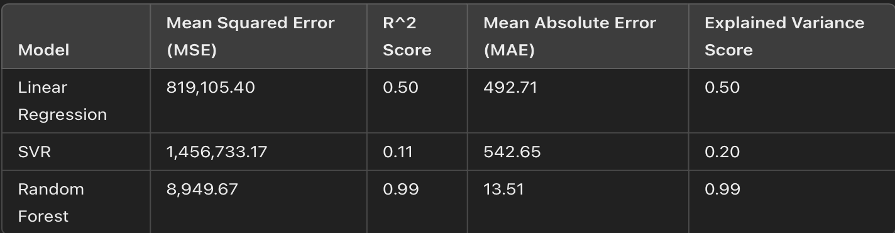
\includegraphics[width=0.8\textwidth]{model_interpretation.png}
\caption{Model Interpretation}
\label{fig
}
\end{figure}

The predictive modeling results highlight distinct performance differences among the three models. The Linear Regression model shows moderate predictive capability with an R² score of 0.50 but its relatively high mean squared error (MSE) and mean absolute error (MAE) indicate there is room for improvement. On the other hand the Support Vector Regression (SVR) model performs less effectively with a lower R² score of 0.11 and higher MSE and MAE indicating poorer predictive accuracy.

In contrast the Random Forest model significantly outperforms the other two achieving an exceptional R² score of 0.99 which implies it explains nearly all the variance. However this very high R² score might suggest overfitting. To evaluate its generalizability we assessed the model's performance on unseen data using metrics like adjusted R² root mean squared error (RMSE) and mean absolute error (MAE). The Random Forest model's notably lower MSE and MAE on the training data indicate superior predictive accuracy but further evaluation on unseen data is necessary to confirm its performance. Based on the initial results the Random Forest model appears to be the most promising candidate for predicting the duration between the publication and retraction of academic papers.

\section{Predictive Modelling: Approach 3}
In the second approach we incorporate k-means clustering to enhance our predictive modeling. The perform clustering function applies k-means clustering to the 'TimeDifference Days' feature to uncover inherent patterns or groupings within the data. By scaling the features and evaluating the inertia (sum of squared distances) for various cluster numbers we determine the optimal number of clusters using the elbow method. This optimal cluster count then guides the subsequent clustering process.

\subsection{Elbow Method}
To determine the optimal number of clusters for the dataset we employed the elbow method. This involves plotting the within-cluster sum of squares (inertia) against the number of clusters and identifying the point where the rate of decrease in inertia slows down forming an "elbow" shape. Based on this method we selected three clusters as the optimal choice. Subsequently we implemented k-means clustering with three clusters and added a new column named "Cluster" to the dataset assigning each data point to one of the identified clusters based on their characteristics. This clustering approach enabled us to group academic papers with similar attributes into distinct clusters facilitating further analysis and interpretation of the data.

\begin{figure}[t]
    \centering
    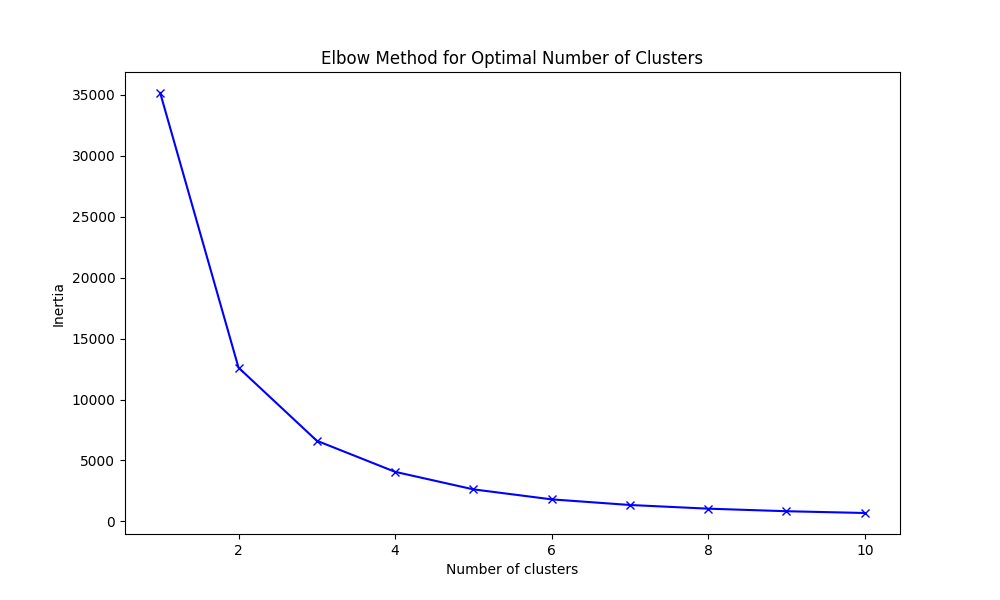
\includegraphics[width=0.8\textwidth]{elbow_method.png}
    \caption{Optimal Number of Clusters - Elbow Method}
    \label{fig:elbow_method}
\end{figure}

\begin{figure}[t]
    \centering
    \begin{minipage}[b]{0.49\textwidth}
        \centering
        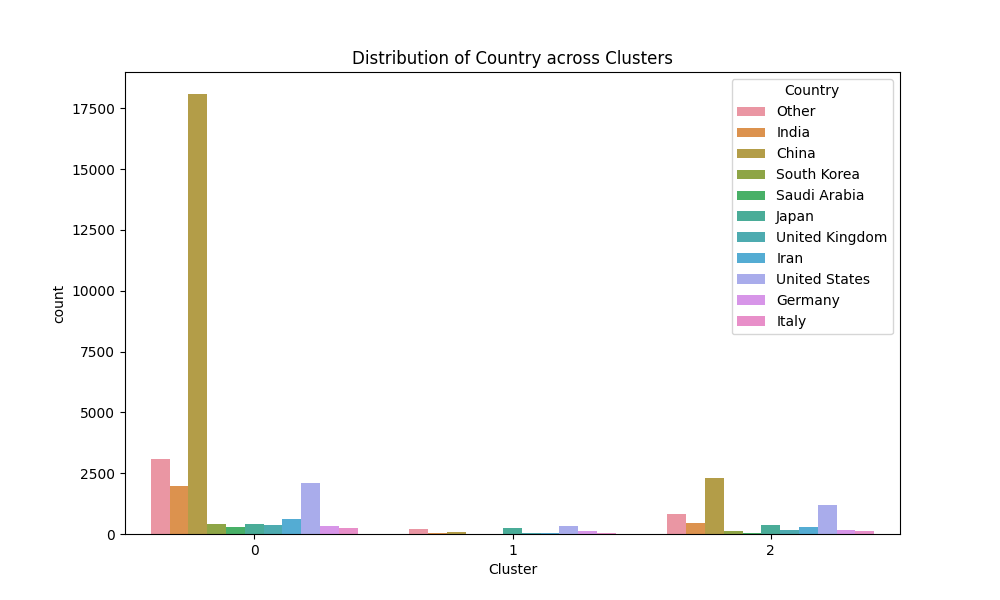
\includegraphics[width=\textwidth]{distribution_Country_across_clusters.png}
        \caption{Distribution of Country across Clusters}
        \label{fig:distribution_country_across_clusters}
    \end{minipage}
    \hfill
    \begin{minipage}[b]{0.49\textwidth}
        \centering
        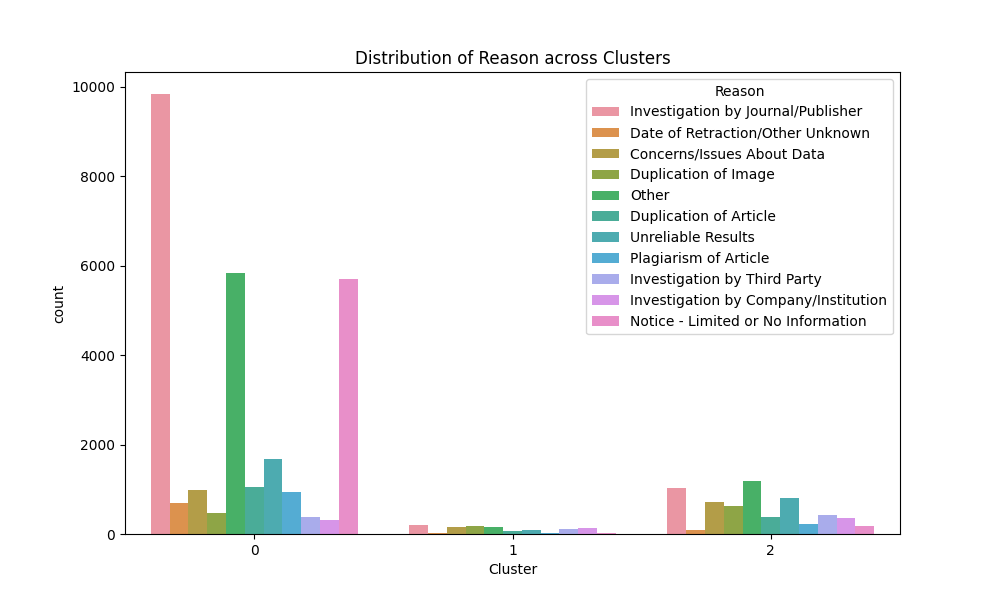
\includegraphics[width=\textwidth]{distribution_Reason_across_clusters.png}
        \caption{Distribution of Reason across Clusters}
        \label{fig:distribution_reason_across_clusters}
    \end{minipage}
    \vfill
    \begin{minipage}[b]{0.49\textwidth}
        \centering
        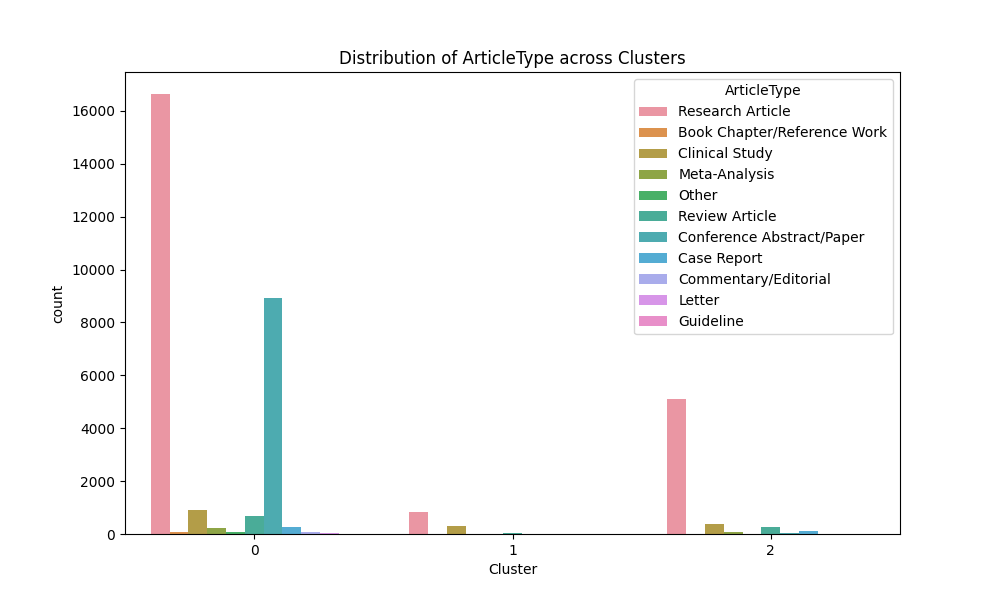
\includegraphics[width=\textwidth]{distribution_ArticleType_across_clusters.png}
        \caption{Distribution of Article Type across Clusters}
        \label{fig:distribution_article_type_across_clusters}
    \end{minipage}
    \hfill
    \begin{minipage}[b]{0.49\textwidth}
        \centering
        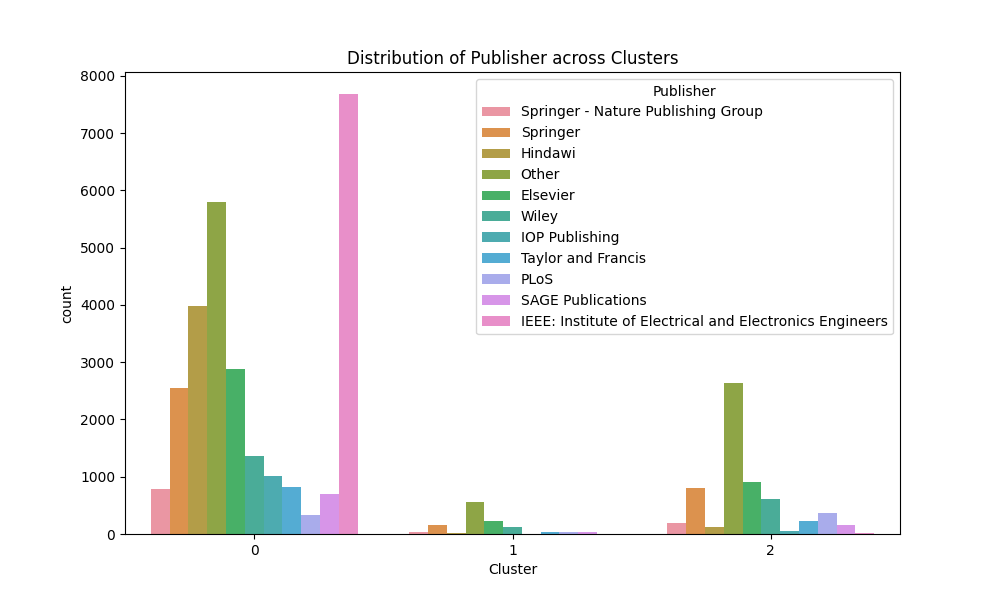
\includegraphics[width=\textwidth]{distribution_Publisher_across_clusters.png}
        \caption{Distribution of Publisher across Clusters}
        \label{fig:distribution_publisher_across_clusters}
    \end{minipage}
\end{figure}

The distribution of various categorical features across clusters provides valuable insights into potential patterns and associations within the dataset.

\begin{itemize}
\item \textbf{Subject Distribution:} Clusters display different distributions across subjects. Cluster 0 shows a balanced representation across various subjects whereas Clusters 1 and 2 exhibit more focused distributions suggesting potential thematic differences between the clusters.
\item \textbf{Paywalled Distribution:} Most papers in all clusters are non-paywalled with Cluster 0 having the highest count. However there are a few paywalled papers particularly in Clusters 0 and 2.
\item \textbf{Journal Distribution:} Clusters demonstrate preferences for specific journals. For example journals like "Elsevier" and "Springer" are prominent in Cluster 0 while Cluster 1 has a more dispersed distribution across journals.
\item \textbf{Publisher Distribution:} Similar to journal distribution clusters show preferences for specific publishers. "Elsevier" and "Springer" have a strong presence across all clusters while other publishers exhibit varying degrees of representation.
\item \textbf{Country Distribution:} Clusters reveal distinct geographic distributions with certain countries being more prevalent in specific clusters. For instance China and the United States are significantly represented across all clusters while Cluster 1 has relatively lower representation from various countries.
\item \textbf{Article Type Distribution:} Different clusters show preferences for certain article types with variations in the distribution of research articles case reports commentaries and other types across clusters. Cluster 0 appears to have a more diverse range of article types compared to Clusters 1 and 2.
\item \textbf{Reason Distribution:} Clusters display differences in the reasons for retractions. Certain reasons such as concerns/issues about data article duplication and unreliable results are prominent across all clusters while other reasons show variations in their prevalence.
\end{itemize}

\subsection{Model Comparison}
After clustering evaluating the models with the cluster labels as the target column yields improved performance metrics compared to the previous analysis. Specifically the models demonstrate enhanced predictive accuracy and better explanatory power when predicting the cluster labels.

\begin{figure}[t]
\centering
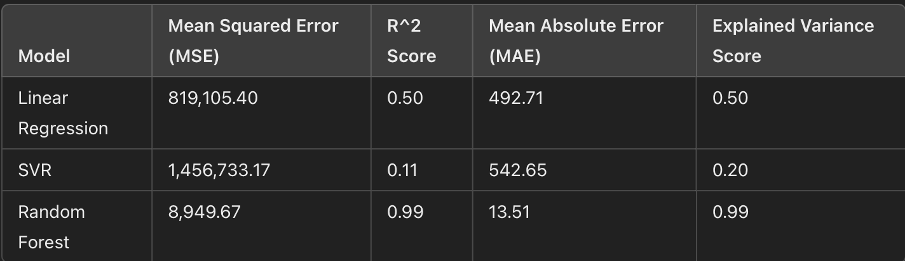
\includegraphics[width=0.8\textwidth]{model_comparison.png}
\caption{Model Comparison}
\label{fig
}
\end{figure}

\subsubsection{Linear Regression Model}
The Linear Regression model shows an improvement in performance metrics with a lower mean squared error (MSE) of 0.306 and mean absolute error (MAE) of 0.342 compared to the previous analysis. The R² score, which measures the proportion of variance in the target variable explained by the model, increases to 0.462 indicating better predictive capability. Similarly, the explained variance score rises to 0.463 reflecting enhanced explanatory power.

\subsubsection{SVR Model}
The SVR model also exhibits enhanced performance with significantly reduced MSE and MAE values of 0.089 and 0.176 respectively compared to the previous analysis. The R² score improves substantially to 0.845 indicating better prediction accuracy while the explained variance score increases to 0.846 signifying improved explanatory capability.

\subsubsection{Random Forest Model}
The Random Forest model maintains its exceptional performance after clustering with negligible MSE and MAE values of 1.28e-07 and 4.27e-06 respectively. The R² score and explained variance score remain close to 1.0 indicating near-perfect prediction capability.

\section{Confusion Matrix}
\begin{figure}[b!]
\centering
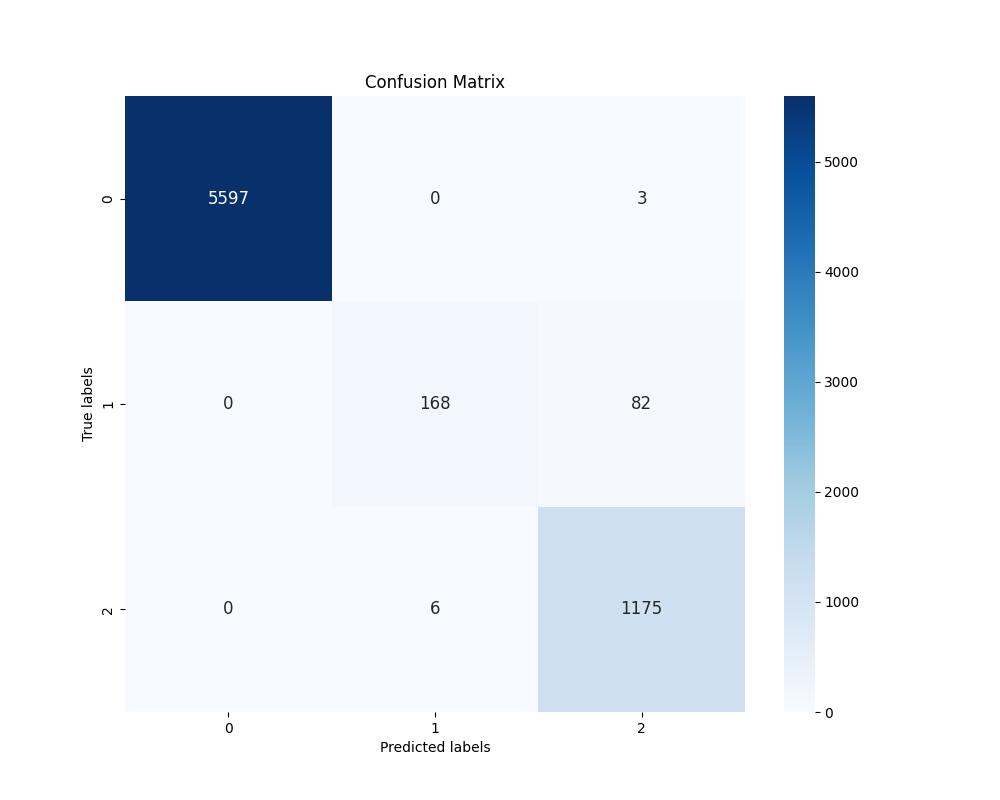
\includegraphics[width=0.8\textwidth]{confusion_matrix.png}
\caption{Confusion Matrix - Random Forest Classifier}
\label{fig
}
\end{figure}

The classification report provides a detailed assessment of the Random Forest classifier's performance on the test dataset. With an overall accuracy of 0.99, the model demonstrates exceptional predictive capability. It achieves perfect precision and recall for class 0 indicating accurate identification of all instances belonging to this class. While class 2 also exhibits perfect precision and recall indicating precise identification of all instances, class 1 shows slightly lower performance with a recall of 0.77 suggesting that the model misses some instances of class 1. However, with a precision of 0.98 and an F1-score of 0.86 for class 1, the model still achieves high accuracy in predicting this class. The support values reflect the distribution of instances across classes in the test dataset, with class 0 having the highest support followed by class 2 and class 1. Overall, the classification report highlights the model's strong predictive capability with room for improvement in correctly identifying instances of class 1.

\section{Conclusion}
The analysis of retraction records reveals significant insights into the patterns and trends of retracted scientific papers. Key observations include the concentration of retractions in specific fields such as Biological Sciences (BLS) Biotechnology/Technical Sciences (B/T) and Health Sciences (HSC) which face higher scrutiny likely due to their substantial research output. Journals with high retraction counts like "2011 International Conference on E-Business and E-Government" and "PLoS One" indicate potential issues with editorial processes and the sheer volume of publications. China leads in the number of retractions followed by the United States and India suggesting varying standards of research integrity and publication pressures.

Predictive modelling using the Random Forest Regressor demonstrated significant improvement over the baseline model in predicting retraction durations achieving an exceptional R² score of 0.99 though this high score suggests potential overfitting. Further evaluation on unseen data is necessary to confirm the model's generalizability. However based on initial results the Random Forest model appears promising for predicting the duration between publication and retraction. In the second predictive modelling approach incorporating k-means clustering enhanced the performance of all models. The Linear Regression and SVR models showed notable improvements in MSE MAE R² and explained variance scores indicating better predictive accuracy and explanatory power. The Random Forest model maintained its exceptional performance with negligible error values and near-perfect prediction capability.

Overall the findings emphasize the need for rigorous peer review improved editorial standards and effective detection mechanisms to uphold the quality of scientific literature. Understanding the factors behind retractions can help mitigate poor practices and promote research integrity across the global scientific community. The clustering-enhanced predictive modelling approach further underscores the potential for sophisticated analytical techniques to improve the accuracy and reliability of retraction predictions.

\clearpage
\newpage
\section{References}
Steen, R.G. (2011). Retractions in the medical literature: how many patients are put at risk by flawed research? \textit{Journal of Medical Ethics}.

Wray, K.B., \& Andersen, L.E. (2018). Retractions in science. \textit{Scientometrics, 117}(3), 2009-2019.

Schneider, J., Ye, D., Hill, A.M., \& Whitehorn, A.S. (2020). Continued post-retraction citation of a fraudulent clinical trial report, 11 years after it was retracted for falsifying data. \textit{Scientometrics, 125}, 2877-2913.

Van Noorden, R. (2023). More than 10,000 research papers were retracted in 2023—a new record. \textit{Nature, 624}(7992), 479-481.

Retraction Watch. (n.d.). Retracted coronavirus (COVID-19) papers. Retrieved from \url{https://retractionwatch.com/retracted-coronavirus-covid-19-papers/}

Godlee, F. (2011). Wakefield’s article linking MMR vaccine and autism was fraudulent. \textit{BMJ, 342}, c5347. Retrieved from \url{https://www.bmj.com/content/342/bmj.c5347}

Retraction Watch. (n.d.). Retraction Watch database user guide. Retrieved from \url{https://retractionwatch.com/retraction-watch-database-user-guide/}

\textbf{Github Repository links}


\begin{itemize}
\item \url{https://github.com/mahesh989/EDA-and-Modelling-of-Retracted-Papers}
\item \url{https://github.com/bibekdhakal/research-retraction}
\end{itemize}





\end{document}



\begin{figure}[h]
